\setchapterstyle{kao}
\setchapterpreamble[u]{\margintoc}
\chapter{Interactive sequents}
\labch{pba}

\begin{kaobox}[frametitle=Note]
  Most of the content in this chapter has been previously published in
  \cite{10.1145/3497775.3503692}.
\end{kaobox}

% \section{What is a sequent?}

% In its original formulation by Gentzen\todo{citation of original paper
% introducing the sequent calculus}, a sequent is simply an expression of the form
% $Γ ⊢ C$, where $\Gamma$ is a list of formulas in the logic of interest, and $C$
% is a distinguished formula. In the context of theorem proving, sequents are
% usually seen as \emph{goals}, a denomination dating back to the LCF prover
% \cite{doi:10.1098/rsta.1984.0067}. That is, the statement $C$ corresponds to the
% \emph{conclusion} the user wants to reach that still needs justification, and
% the latter can be achieved by using either \emph{hypotheses} in $\Gamma$, or
% already proved lemmas stored in a global environment\sidenote{From a purely
% proof-theoretical point of view, having a separate global environment is
% unnecessary, and every statement considered justified --- either proved or
% assumed --- can be put in the hypotheses $Γ$.}.

% One can find a number of extensions and variants to the syntax of sequents,
% depending on the logic under consideration. For example, it is customary in
% propositional and predicate logic to describe $Γ$ as a set or multiset, because
% the way hypotheses are ordered is immaterial with regard to provability.

% However many modern proof assistants are based on \emph{dependent type theory},
% where hypotheses have explicit \emph{names} identifying them, corresponding to
% \emph{variables}. Then sequents have the form $x_1 : A_1, …, x_n : A_n ⊢ C$, and
% oftentimes the type $A_i$ of some hypothesis will refer to variables in $x_1, …,
% x_n$, thus creating dependencies between hypotheses. In this case, one wants to
% avoid dependency cycles by forcing $A_i$ to refer only to previously occuring
% variables $x_j$ where $j < i$, hence the order of hypotheses becomes logically
% meaningful. From a usability point of view, it can also be beneficial to let the
% user reorganize hypotheses in the order she deems most readable in the course of
% a proof.

% Another common feature consists in extending $Γ$ with \emph{definitions} of the
% form $x := b : A$, where $b$ is some term \emph{provably} of type
% $A$\sidenote{This type-theoretical encoding of definitions dates back to the
% work of N. G. De Bruijn on Automath, according to \cite{geuvers_proof_2009}.}.
% Then $x$ acts as a name for the body $b$ of the definition, and is not just
% assumed to be of type $A$. The more neutral word \emph{context} is usually
% preferred over the word \emph{hypotheses} to denote this mixed list of
% assumptions and definitions. It is also common to qualify the definitions in
% $\Gamma$, or even the full context $\Gamma$, as being \emph{local}, to
% distinguish them from the \emph{global} environment of lemmas and definitions
% mentioned earlier.

% We mention one last possible variation, which is to replace the conclusion $C$
% by a list of conclusions $Δ$, which ought to be understood \emph{disjunctively}.
% That is, a sequent $Γ ⊢ Δ$ seen as a goal can be read ``at least one of the
% conclusions in Δ must be proved under the context $Γ$''. Although introduced
% originally by Gentzen in the context of classical logic, this syntax can also be
% used for intuitionistic logics, for example to implement efficient proof search
% procedures \cite{dyckhoff_contraction-free_1992}. In practice however, we do not
% know of any existing proof assistant using multi-conclusion goals at the user
% interface level.


In this chapter, we focus on how both \emph{click} and \emph{drag-and-drop}
(DnD) actions upon the formulas of a sequent can implement proof construction
operations corresponding to the core logic; that is how they deal with logical
connectives, quantifiers and equality. We present these core principles through
various illustrations and examples in first-order logic. The technical and
proof-theoretical foundations for the semantics of DnD actions, which constitute
the main innovation of this work, will be investigated more thoroughly in
\refch{pbl}, although the most important meta-theoretical properties will be
exposed here with outlines of their proofs. More advanced features of the
proof-by-action paradigm that go beyond the core logic, as well as its
integration in a mainstream proof assistant, are presented in \refch{beyond}.

We have started to implement the paradigm in a prototype named {\em Actema} (for
Active Mathematics) running through a web HTML5/JavaScript interface. At the
time of writing, an online version of the prototype can be accessed at
\url{https://actema.xyz/}\marginnote[120pt]{\textbf{TODO:} Have a more durable
way to access the prototype? More generally, what is the correct way to
incorporate software artifacts in a thesis?}. This possibility to experiment in
practice, even though yet on a small scale, gave valuable feedback for crafting
the way DnD actions are to be translated into proof construction steps in an
intuitive and practical way. A description of the overall architecture and
implementation design of Actema will be provided in \refch{beyond}.

The chapter is organized as follows. \refsec{setting} briefly outlines its
logical setting. \refsec{aristote} describes the basic features of a graphical
proof interface based on our principles, and illustrates them with a famous
syllogism from Aristotle. \refsec{clicks} shows how it can integrate basic
proof-by-pointing capabilities. \refsec{newitems} shows very briefly how one can
add new formulas and objects to the current goal. The next two sections explain,
through further examples, how drag-and-drop actions work; first for
so-called \emph{rewrite} actions involving equalities, then for actions
involving logical connectives and quantifiers. \refsec{soundness} introduces
the notions of context and polarity, in order to prove the soundness of our
system. \refsec{linkages} explains how DnD actions are specified by the user
interactively, through schemas called \emph{linkages}. \refsec{action} describes
how linkages translate into logical steps, and sections \ref{sec:productivity}
and \ref{sec:invert} discuss some properties of this translation.
\refsec{edukera} studies a proof of a small logical riddle in Actema,
highlighting some benefits of our approach compared to textual systems. We end
with a discussion on some related works in \refsec{related-work}.

% \section{Motivations}\labsec{motivations} Since this work is about changing
% the very way the user interacts with an interactive theorem prover, we feel it
% is important to make some disclaimers about the aims and the scope of what is
% presented here.

% From a development point of view, we are still at a very preliminary
% stage. Building a real-size proof system integrating the ideas we
% present would require an important effort and is still a long term
% goal. Some concepts however have emerged, which, we hope allow to
% sketch some aspects of the look-and-feel of such a system, and what
% some of its advantages could be.

% Also, at this stage, we focus on basic proof constructions and on how the
% gestural approach can help make them more efficient and more intuitive. Some of
% the illustrative examples we give below could probably be dealt with using
% advanced proof search tactics, but we believe this does not make them
% irrelevant. Rather than (sub)goals to be proved, these examples should be seen
% as generic situations often encountered in the course of a proof, which require
% small and local transformations to the statements involved.
% % Indeed, one objective of our approach is to provide users with fine-grained
% % control over the shape of the proof state, through a small set of basic
% % interaction principles. 

% The idea of interactive theorem provers is that automation and user actions
% complement each other, and we here focus on the latter for the time being. The
% question of integrating drag-and-drop actions and powerful proof automation
% techniques is left for future work.

% Finally, precisely because our approach is about giving the user a smoother
% control of the proof construction process, we see a possibility for
% our work to help making future proof systems more suited for education.

\section{Logical Setting}\labsec{setting}
Any proof system must implement a given logical formalism. What we
describe here ought to be applied to a wide range of formalisms, but
in this chapter we focus on the core of intuitionistic first-order logic
with equality (FOL). This allows us to consider sequents where
hypotheses are unordered which, in turn, simplifies the technical
presentation.  We will thus write $\Gamma,A \seq C$ for a sequent
where $A$ is among the hypotheses.

We use and do not recall the usual definitions of terms and propositions in
first order logic. We assume a first order language (function and predicate
symbols) is given. Provability is defined over sequents $\Gamma\seq C$ by the
usual logical rules of natural deduction (\sys{NJ}) and/or sequent calculus
(\sys{LJ}), as defined in \refch{proof-theory}.

Equality is treated in a common way: $=$ is a binary
predicate symbol written in the usual infix notation, together with the
reflexivity axiom $\forall x.x=x$ and the Leibniz scheme, stating that for any
proposition $A$ one has
$$\forall x.\forall y. x=y\land A \limp \subst{A}{x}{y}.$$

\begin{figure*}
 \begin{center}
\fbox {   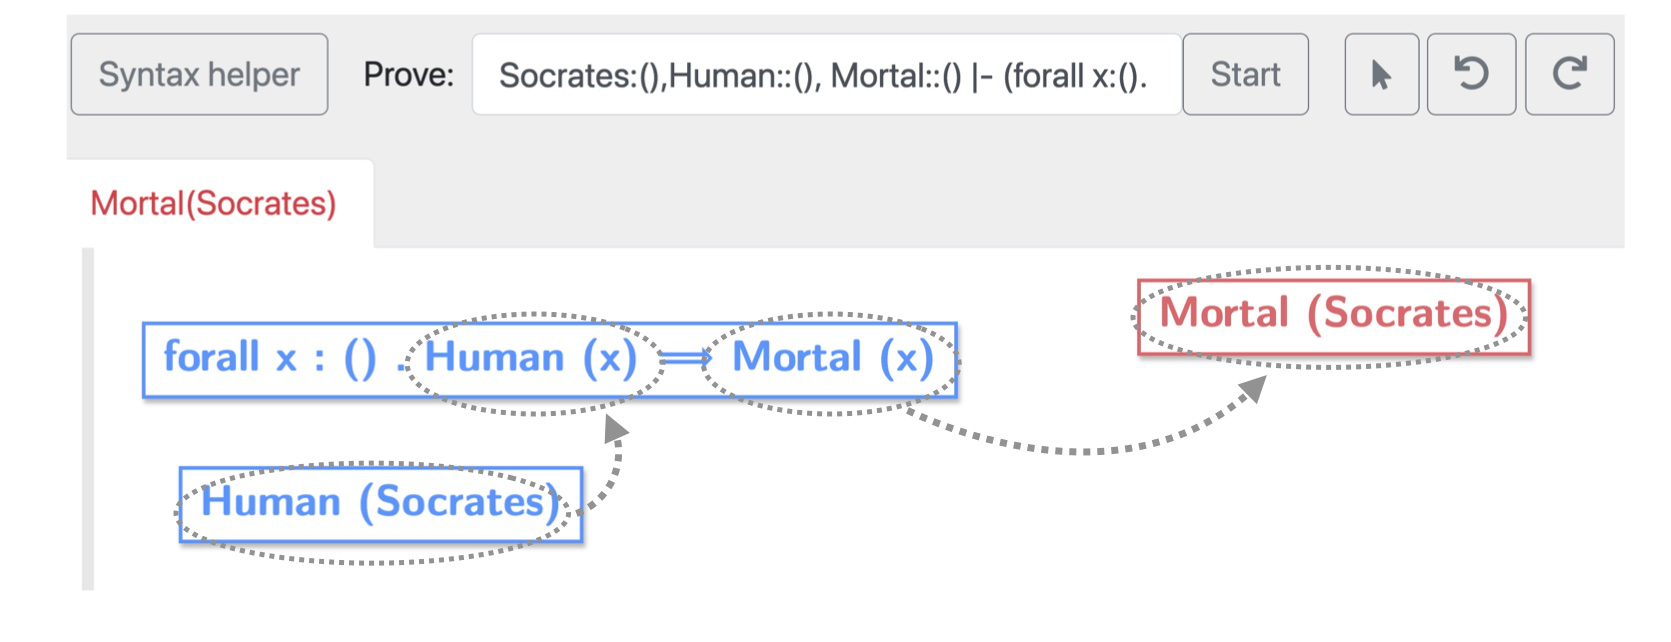
\includegraphics[width=1.3\textwidth]{actions-tag.png}}
 \end{center}
 \caption{A partial screenshot showing a goal in the Actema prototype}
 The conclusion is red on the right, the two hypotheses blue on the left. The
   grey dotted arrows have been added to show the two possible actions.
 \labfig{aristote}
 \end{figure*}

We will not consider, on paper, the details of variable renaming in
substitutions, implicitly applying the so-called Barendregt
convention, that bound and free variables are distinct and that a
variable is bound at most once.

Extending this work to simple extensions of FOL, like multi-sorted predicate
calculus is straightforward (and actually done in the Actema prototype).  Some
interesting points may show up when considering how to apply this work to more
complex formalisms like type theories. We will not explore these questions here.

Another interesting question is how our approach extends to classical logic(s),
by using multi-conclusion sequents. In this chapter we only give a few hints on
this topic. A more thorough investigation will be done in
\refsec{sfl-classical}.

\section{A First Example}\labsec{aristote}

\subsection{Layout}
One advantage of the proof-by-action paradigm, is that it allows a very lean
visual layout of the proof state. There is no need to name hypotheses. In the
prototype we also dispense with a text buffer, since proofs are solely built
through graphical actions.


\reffig{aristote} shows the layout of the system using the
ancient example from Aristotle. A goal appears as a set of {\em items}
whose nature is defined by their respective colors\sidenote{We are
  well aware that, in later implementations, this color-based
  distinction ought to be complemented by some other visual
  distinction, at least for users with impaired color vision. But in
  the present description we stick to the red/blue denomination, as it
  is conveniently concise.}:
\begin{itemize}
\item A {\em red item} which is the proposition to be proved, that is the
 {\em conclusion},
\item {\em blue items}, which are the local {\em hypotheses}.
\end{itemize}

{\em The items are what the user can act upon: either by {\em clicking} on
them, or by {\em moving} them.}

Finally, note that each goal is displayed on a tab.

\subsection{Two Kinds of Actions}
In this example, there are two possible actions.

\begin{itemize}
\item A first one is to bring together, by drag-and-drop, the red conclusion
$\mortal(\socrates)$ with the succedant of the first hypothesis $\mortal(x)$.
This will transform the goal by changing the conclusion to $\human(\socrates)$.
\item A second possibility is to combine the two hypotheses; more precisely to
bring together the item $\human(\socrates)$ with the premise $\human(x)$ of the
first hypothesis. This will yield a new hypothesis $\mortal(\socrates)$.
\end{itemize}

The first case is what we call a {\em backward step} where the conclusion is
modified by using a hypothesis. The second case is a {\em forward step} where
two known facts are combined to deduce a new fact, that is an additional blue
item.

In both cases, the proof can then be finished invoking the logical
axiom rule. In practice this means bringing together the blue
hypothesis $\human(\socrates)$ (resp. the new blue fact
$\mortal(\socrates)$) with the identical red conclusion.


\subsection{Modelling the Mechanism}

A backward step involves a hypothesis, here $\forall x.\-\human(x)
\allowbreak\limp \mortal(x)$ and the conclusion, here $\mortal(\socrates)$.
Furthermore, the action actually links together two {\em subterms} of each of
these items; this is written by squaring these subterms. The symbol ${\back}$,
used as an operator, is meant to describe the result of the interaction.
Internally, the behavior of this operator is defined by a set of rewrite rules
given in \reffig{DISL} and \reffig{DISL-U}. Here is the sequence of
rewrites corresponding to the example\sidenote{Note that $\back$ has lower
precedence than all logical connectives.}: \renewcommand{\arraystretch}{1.1}
$$\begin{array}{lll}
    &  \forall x.\human(x)\limp \select{\mortal(x)} \back \select{\mortal(\socrates)}&\\
    \step &
           \human(\socrates)\limp \select{\mortal(\socrates)}
           \back \select{\mortal(\socrates)}&
                                               \mathsf{L\forall i}\\
    \step &
           \human(\socrates)\land(\select{\mortal(\socrates)}
           \back \select{\mortal(\socrates)}) &
                                                 \mathsf{L\!\!\limp_2}\\
    \step &  \human(\socrates)\land \top &
                                           \mathsf{id}\\
    \step & \human(\socrates)&\mathsf{neur}\\
  \end{array}$$

Notice that:
\begin{itemize}
\item   These elementary rewrites are not visible for the user. What she sees is
  the final result of the action, that is the last expression of the rewrite
  sequence.
\item The definitions of the rewrite rules in \reffig{DISL} and
  \reffig{DISL-U} do not involve squared subterms. The information of which
  subterms are squared is only used by the system to decide which rules to
  apply in which order.
\end{itemize}

In general, the action solves the goal when the interaction ends with
the trivially true proposition $\top$. The base case being the action
corresponding to the axiom/identity rule \rnmsf{id}: $A\back A \step\top$.

A forward step, on the other hand, involves two (subterms of two)
hypotheses. The interaction operator between two hypotheses is written
$\forw$. In the example above, the detail of the interaction is:
$$
  \begin{array}{lll}
    &  \forall x .\select{\human(x)}\limp\mortal(x) \forw \select{\human(\socrates)}&\\
    \step & \select{\human(\socrates)}\limp\mortal(\socrates) \forw \select{\human(\socrates)}& \mathsf{F \forall i}\\
    \step & (\select{\human(\socrates)}\back \select{\human(\socrates)} )\limp\mortal(\socrates) &\mathsf{F\!\!\limp_1}\\
    \step & \top \limp\mortal(\socrates) &\mathsf{id}\\
    \step & \mortal(\socrates) & \mathsf{neul}\\
  \end{array}
$$

The final result is the new hypothesis. We come back to the study of the rewrite
rules of ${\back}$ and ${\forw}$ further down.


\section{Proof Steps through Clicks}\labsec{clicks}
Drag-and-drop actions involve two items. Some proof steps involve only
one item; they can be associated to the action of clicking on this
item. The general scheme is that clicking on a connective or quantifier
allows to ``break'' or destruct this connective. The results of clicks
are not very surprising, but this feature is necessary to complement
drag-and-drop actions.
\begin{itemize}
\item Clicking on a blue conjunction $A\land B$ transforms the
    item into two separate blue items $A$ and $B$.
\item Clicking on a red conjunction $A\land B$ splits the goal into
    two subgoals, whose conclusions are respectively $A$ and $B$.
\item Clicking on a blue disjunction $A\lor B$ splits the goal into two subgoals
    of same conclusion, with $A$ (resp. $B$) added as a new hypothesis.
\item Clicking on the left (resp. right)-hand subterm of a red
      disjunction $A\lor B$ replaces this red conclusion by $A$
      (resp. $B$).
\item Clicking on a red implication $A\limp B$ breaks it into a
      new red conclusion $B$ and a new blue hypothesis $A$.
\item Clicking on a red universal quantifier $\forall x.A$ introduces
  a new object $x$ and the conclusion becomes $A$.
\item Clicking on a blue existential $\exists x.A$ introduces a new
  object $x$ together with a blue hypothesis $A$.
\item Clicking on a red equality $t = t$ solves the goal immediately.
\end{itemize}

One can see that these actions correspond essentially to the (right)
introduction rules of the head connective for the conclusion, and either the
elimination rule from \sys{NJ} or the left introduction rule from \sys{LJ} for
hypotheses. The exact mapping between click actions and inference rules is
given in \reftab{click-rules}. A few remarks are in order:
\begin{itemize}
  \item In the current implementation of Actema, clicking on a blue item $A
  \limp B$ will work only if the conclusion is $B$. An alternative is to use the
  {\rnmsf{{\limp}L}} rule from sequent calculus, which is applicable in every
  context.
  \item There is no action mapped to red $\bot$ items, simply because $\bot$
  does not have any introduction rule.
  \item There is currently no action mapped to blue $∀$ and red $∃$ items. The
  reason is that one needs additional information about the \emph{witness} to be
  used when instantiating with the $∀L$ or $∃R$ rule. This could be provided
  with further input (e.g. from a dialog box), but this would need a change in
  the communication protocol between the frontend and backend of Actema. Instead
  we decompose this in two steps: first the user can add the witness as a new
  object by using the \texttt{+expr} button (see \refsec{newitems}); then she
  can drag the corresponding green item and drop it on the quantified item to
  instantiate it. It is also possible to select with the mouse an arbitrary
  subexpression occurring in any item of the current goal, and then
  drag-and-drop the item holding the selected subexpression instead.
\end{itemize}

\begin{table}[]
\caption[]{Mapping of click actions to inference rules}
\labtab{click-rules}
\begin{tabular}{ccc}
	\toprule
	\thead{Head connective} & \thead{Red item} & \thead{Blue item} \\
	\midrule
  $\top$ & \rnmsf{\top R} & \rnmsf{\top L} \\
	\midrule
  $\bot$ & $\emptyset$ & \rnmsf{\bot L} \\
	\midrule
	$\land$ & \rnmsf{\land R} & \rnmsf{\land L} \\
	\midrule
	$\lor$ & \rnmsf{\lor R_1, \lor R_2} & \rnmsf{\lor L} \\
	\midrule
  $\limp$ & \rnmsf{{\limp}R} & \rnmsf{{\limp}E} \\
	\midrule
  $∀$ & \rnmsf{∀R} & $\emptyset$ \\
	\midrule
  $∃$ & $\emptyset$ & \rnmsf{∃L} \\
	\bottomrule
\end{tabular}
\end{table}


It is possible to associate some more complex effects to click actions performed
on locations deeper under connectives. This is the essence of proof-by-pointing,
and~\cite{PbP} provides ample description. Since we here focus on drag-and-drop
actions, we do not detail further more advanced PbP features. However we stress
that these features are essentially compatible with what we describe in this
work. In fact the version of Actema presented in \refch{beyond} provides an
implementation of proof-by-pointing available as a contextual menu action.

\section{Adding New Items}\labsec{newitems}

Often in the course of a proof, one will want to add new items: either a new
conjecture (blue item), or a new object (green item) that would be helpful to
solve the current goal. These can be done respectively with the blue
\texttt{+hyp} and the green \texttt{+expr} buttons, which appear in the
screenshot of \reffig{edukera}. When clicked, they prompt the user
for the statement of the conjecture, or the name and expression defining the
object. The \texttt{+hyp} button will also create a new subgoal requiring to
prove the conjecture within the current context.

This mechanism and the syntax are for now very crude. The design of
possible smoother tools is an important issue but left for future
work\sidenote{For instance~\cite{omar-filling-2021} deals with a
  similar problem in the context of functional programming.}.

% Currently we ask the user to input textual data, in an idiosyncratic syntax
% specific to the logic of the Actema prototype. A desirable, but highly
% non-trivial feature would be to provide some elaborate input mechanism tailored
% for the type of object the user wants to create. This would obviously require
% some extensibility to new domain-specific input interfaces, which lies outside
% the scope of this article\sidenote{For a related work that tackles this problem
% in the context of functional programming, see e.g. \cite{omar-filling-2021}}.
% Note however that it seems like a necessary feature if one wants to achieve a
% fully graphical theorem proving environment.

\section{A Simple Example Involving Equality}\labsec{equality}

Most interactive theorem provers expose a \emph{rewrite} tactic that allows the
use of equality hypotheses, that is known equations of the form $t = u$, in
order to replace some occurrences of $t$ by $u$ (or symmetrically, occurrences
of $u$ by $t$). This substitution can be performed in the conclusion or in
hypotheses. Specifying the occurrences to be replaced with textual commands can
be quite tedious, since it involves either dealing with some form of
naming/numbering to designate locations of subterms, or writing manually
patterns which duplicate parts of the structure of terms.

\begin{figure*}
  \begin{center}
    \fbox{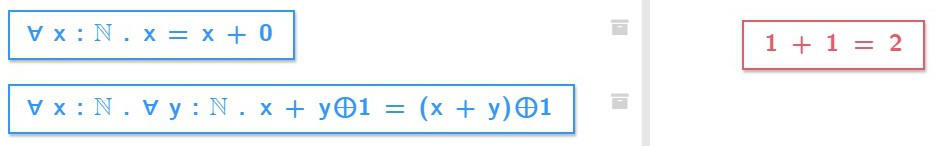
\includegraphics[width=1.3\textwidth]{oneplusone.png}}
  \end{center}
  \caption{Proving $1 + 1 = 2$ in Peano arithmetic}
  \labfig{oneplusone}
\end{figure*}

In our setting we can provide this replacement operation through
drag-and-drop. The user points at the occurrence(s) of $t$ to be
replaced, and then brings them to the corresponding side of the
equality.

\reffig{oneplusone} shows a very elementary example where one wants to
prove $1+1=2$ in the setting of Peano arithmetic. For any number $n$, we write
$\suc{n}$ to denote the application of the successor function to $n$; closed
terms are directly written in decimal notation. The proof goes as
follows\sidenote{We use the symbol $\syneq$ to denote syntactic equality of two
expressions modulo \emph{pretty-printing}, e.g. decimal notation.}:
\begin{itemize}
  \item We link the left-hand side $x + \suc{y}$ of the second addition axiom with $1 + 1$ in the conclusion, which has the effect of rewriting $1 + 1$ into $\suc{(1 + 0)}$:
    $$
      \begin{array}{lll}
        & \forall x. \forall y. \select{x + \suc{y}} = \suc{(x + y)} \back \select{1 + 1} = 2 & \\
        \step & \forall y. \select{1 + \suc{y}} = \suc{(1 + y)} \back \select{1 + 1} = 2 &\mathsf{L\forall i} \\
        \step & \select{1 + \suc{0}} = \suc{(1 + 0)} \back \select{1 + 1} = 2 &\mathsf{L\forall i} \\
        \syneq & \select{1 + 1} = \suc{(1 + 0)} \back \select{1 + 1} = 2 & \\
        \step & \suc{(1 + 0)} = 2 &\mathsf{L\!\!=_1}
      \end{array}
    $$
  \item We link the right-hand side $x + 0$ of the first addition axiom with $1 + 0$ in the conclusion, which rewrites $1 + 0$ into $1$:
    $$
      \begin{array}{lll}
        & \forall x. x = \select{x + 0} \back \suc{(\select{1 + 0})} = 2 & \\
        \step & 1 = \select{1 + 0} \back \suc{(\select{1 + 0})} = 2 &\mathsf{L\forall i} \\
        \step & \suc{1} = 2 &\mathsf{L\!\!=_2} \\
        \syneq & 2 = 2 &
      \end{array}
    $$
\end{itemize}

We end up with the conclusion $2 = 2$, which is provable by a simple click.
Notice how the orientation of the two rewritings is determined by which side of
the equality is selected. Also, in this case, the rewritings
correspond to backward proof steps, because the rewriting is performed
in the conclusion. Similar rules (\rnmsf{F\!\!=_1} and \rnmsf{F\!\!=_2}) are
used to perform rewritings in hypotheses.


\section{Drag-and-Dropping through Connectives}\labsec{dnd-examples}
We mentioned in \refsec{clicks} that it is possible to destruct logical
connectives through click actions. In many cases however, this will not be
necessary: because a drag-and-drop involves subterms of the items involved, one
can often directly use (resp. act on) the part of the hypothesis (resp.
conclusion) which is of interest.

\subsection{Conjunction and Disjunction}
The conjunction is an easy to explain case. A hypothesis of the form
$A\land B$ can be used directly both as evidence for $A$ and as evidence
for $B$. This is modeled by the rules \rnmsf{L\land_1} and
\rnmsf{L\land_2}. A very simple action is thus:
$$
\begin{array}{llll}
  \select{A}\land B \back \select{A} & \step& \select{A} \back
  \select{A} \hbox to 1cm {\hfil}&\mathsf{L \land_1}\\
                                       & \step &\top & \mathsf{id}
\end{array}
$$

On the other hand, considering a conjunctive goal $A\land B$, one can
simplify or solve one of the branches by a DnD action. This involves
rules \rnmsf{R \land_1} and
\rnmsf{R \land_2}. For instance:
$$
\begin{array}{llll}
  \select{A} \back \select{A}\land B &
                                         \step& (\select{A} \back
                                         \select{A})\land B &\mathsf{R \land_1}\\
                                       & \step& \top \land B  & \mathsf{id}\\
  &\step& B&\mathsf{neul}
\end{array}
$$

Red disjunctions work similarly to conjunctive goals, except that solving one
branch will solve the entire goal. A nice consequence of this, which is hard to
simulate with textual tactics, is that one can just simplify one branch of a
disjunction without comitting to proving it entirely:
$$
\begin{array}{llll}
  \select{A} \back (B \land \select{A}) \lor C
    & \step & (\select{A} \back B \land \select{A}) \lor C &\mathsf{R\lor_1}\\
    & \step & (B \land (\select{A} \back \select{A})) \lor C &\mathsf{R\land_2}\\
    & \step & (B \land \top) \lor C &\mathsf{id}\\
    & \step & B \lor C &\mathsf{neur}
\end{array}
$$

Disjunctive hypotheses also have a backward behavior defined by the rules
\rnmsf{L\lor_1} and \rnmsf{L\lor_2}, although in most cases one will prefer the
usual subgoal semantics associated with click actions. More interesting is
their forward behavior with the rules \rnmsf{F\lor_1} and \rnmsf{F\lor_2}, in
particular when they interact with negated hypotheses. For instance:
$$
\begin{array}{llll}
  \select{A} \lor B \forw \neg \select{A}
    & \step & (\select{A} \forw \neg\select{A}) \lor B &\mathsf{F\lor_1}\\
    & \step & \neg (\select{A} \back \select{A}) \lor B &\mathsf{F\!\!\limp\!\!_1}\\
    & \step & \neg \top \lor B &\mathsf{id}\\
    & \step & \bot \lor B &\mathsf{neul}\\
    & \step & B &\mathsf{neul}\\
\end{array}
$$

We have noticed that on some examples, such actions could provide a
significant speed-up with respect to traditional textual command
provers. We give a more concrete example in \refsec{edukera}.

Notice that we used rules associated with implication, since negation can be
defined by $\neg A \triangleq A \limp \bot$.

\subsection{Implication}\labsec{implication}
The implication connective is crucial, because it is not monotone. More
precisely, the roles of hypotheses and conclusions are reversed on the
left of an implication. We start with some very basic examples
for the various elementary cases.

Using the right hand part of a hypothesis $A\limp B$ turns a 
conclusion $B$ into $A$. 
$$
\begin{array}{llll}
  A\limp \select{B} \back \select{B} &\step& A\land (\select{B}
                                                \back
                                                \select{B})&\mathsf{L
                                                             \!\!\limp_2}\\
                                         &\step&A\land\top & \mathsf{id}\\
    &\step& A&\mathsf{neul}
\end{array}
$$

This can also be done under conjunctions and/or disjunctions:
$$
  A\limp \select{B} \back C \land (D\lor \select{B}) ~~ \steps ~~ C \land (D\lor A)
$$

An interesting point is what happens when using implications with
several premisses. The curried and uncurried versions of the
implication will behave exactly the same way:

$$
  A\limp B \limp \select{C} \back D\lor \select{C}
  ~~~\/ ~\steps~~~  D\lor (A\land B)
$$
and:
$$
  A\land B \limp \select{C} \back D\lor \select{C}
  ~~~ \/ ~\steps~~~  D\lor (A\land B)
$$


As we have seen in Aristotle's example (\refsec{aristote}), blue
implications can also be used in forward steps, where another
hypothesis matches one of their premisses.

A first nice feature is the ability to strengthen a hypothesis by
providing evidence for any of its premises:
$$
B\limp \select{A}\limp C \forw \select {A}  ~~\/~\/~\steps~\/~~~~~
B\limp C$$
and again the same can be done for the uncurryfied version:
$$
B\land \select{A}\limp C \forw \select {A}  ~\/~\/~\steps~\/~~~~~
B\limp C.$$

The two aspects of the implication can be combined:

$$
B\limp \select{A}\limp C \forw D\limp\select {A}  ~\/~\/~\steps~\/~~~~~
B\limp D\limp C$$
or:
$$
B\land \select{A}\limp C \forw D\limp\select {A}  ~\/~\/~\steps~\/~~~~~
B\land D \limp C.$$


Note that there is almost no difference in the way one uses different
versions of a hypothesis $A\limp B\limp C$, $A\land B\limp
C$, but also $B\limp A\limp C$, in forward as well as in
backward steps\sidenote{When viewed as types through the Curry-Howard
isomorphism, $A\limp B\limp C$, $A\land B\limp C$, $B\land
A\limp C$ and $B\limp A\limp C$ are {\em isomorphic types};
and Roberto di Cosmo~\cite{ISOSBook} has also precisely underlined
that type isomorphisms should help to free the programmer from
arbitrary syntactical choices.}. This underlines, we hope, that our
proposal makes the proof construction process much less dependent on
arbitrary syntactical details, like the order of hypotheses or whether
they come in curryfied form or not.

Also, the rules for implication combined with the rules for equality
\rnmsf{L\!\!=_i} or \rnmsf{F\!\!=_i} naturally give access to {\em
  conditional rewriting}; we detail this in combination with
quantifiers in the next section.

%A powerful property of our rewrite rules is that this behavior is true at
%\emph{any depth} under logical connectives.


As for red implications, they also have a backward semantics with the rules
\rnmsf{R\!\!\limp\!\!_1} and \rnmsf{R\!\!\limp\!\!_2}, but most of the time one
will want to destruct them immediately by click. An exception could be if one
wants to simplify some part of an implicative, inductive goal before starting
the induction.

\subsection{Quantifiers}
As the first example of this chapter shows, drag-and-drop actions work through
quantifiers and can trigger instantiations of quantified variables. This is made
possible by the rules \rnmsf{L\forall i} and \rnmsf{F\forall i}, which allow the
instantiation of a variable universally quantified in a hypothesis.

Symmetrically, a variable quantified existentially in a conclusion can
also be instantiated. For instance:

$$\begin{array}{llll}
    \select{A(t)}\back \exists x.\select{A(x)}&\step&
                                                      \select{A(t)}\back\select{A(t)}&\mathsf{L}\forall\mathsf{i}
    \\
                                               &\step& \top&\mathsf{id}
  \end{array}
  $$

An interesting feature is the possibility to modify propositions under
quantifiers. Consider the following possible goal:
% Take this example involving equality:
% $$\begin{array}{clc}
%    & \forall x.\select{ x+0 = x }\back \forall a. \select{a+0} = 0 +
%      a&  \\
%          \step&\forall a.(\forall x.\select{x+0 = x }\back \select{a+0} =
%             0 +a)&\mathsf{R}\forall\mathsf{s}\\
%      \step&\forall a. (\select{a+0=a}\back  \select{a+0} = 0 +a)& \mathsf{L}\forall\mathsf{i}\\
%      \step&\forall a. a = 0+a&\mathsf{L}=1
%                                \end{array}$$
% Performing such a transformation of the goal $\forall a.a+0=0+a$
% without destroying the head quantifier is not trivial traditional
% provers; here it is done through one simple action.
$$\forall a.\exists b. A(f(a)+g(b))$$
where $A$, $f$ and $g$ can be complex expressions. Suppose we have a
lemma allowing us to prove:
$$\forall a.\exists b. A(g(b)+ f(a)).$$
Switching from one formulation to the other, involves one use of the
commutativity property $\forall x.\forall y. x+y=y+x$.
% But because this has to be performed under two quantifiers, doing this in
% traditional interactive theorem provers can be tedious. For instance in Coq, one
% must use a specific tactic called \texttt{setoid_rewrite}.
In our setting, the equality can be used under quantifiers in one single action:
$$
\begin{array}{ll}
  &\forall x.\forall y. \select{x+y}=y+x \back \forall a.\exists b. A(\select{f(a)+g(b)})\\
\steps & \forall a.\exists b. A(g(b)+f(a))
\end{array}$$


Note also that it is possible to instantiate only some of the universally
quantified variables in the items involved. In general, a universally
quantified variable can be instantiated when the quantifier is in a
negative position; for instance:
%\setlength{\abovedisplayskip}{-5pt}
%\setlength{\belowdisplayskip}{0pt}
%\setlength{\belowdisplayshortskip}{0pt}
$$
\begin{array}{rcl}
 \forall x.\forall
 y. \select{P(y)}\limp R(x,y)\forw \select{P(a)} ~\/~\steps
~\/~ \forall x. R(x,a)
 %% \\
 %% \mbox{\hbox to 0pt{\hss or equivalently:}}
 %% \forall y.\forall
 %% x. \select{P(x)}\limp R(x,y)\forw \select{P(a)} \steps
 %% \forall y. R(a,y)
\end{array}
$$
This last example illustrates how partial instantiation abstracts away the order
in which quantifiers are declared, very much like the partial application
presented earlier for implication\sidenote{This fact should not be too
surprising to readers familiar with dependent type theory, where implication is
usually defined as a special case of universal quantification.}.
%% What the last example stresses is, again, that syntactical details,
%% here the order in which variables are quantified, are much less
%% relevant in the gestual proof constructions than in their textual
%% counterparts.


Again, in some cases, only some existential quantifiers may be
instantiated following a linkage:
$$
\begin{array}{rcl}
\select{P(a)}\back \exists x.\exists y. \select{P(y)}\land R(x,y)
 ~\/~\steps
~\/~
    \exists x. R(x,a)
\end{array}
$$

When using an existential assumption, one can either destruct it
through a click, or use or transform it through a DnD; for instance:
$$
\exists x.\select{P(x)}\forw \forall y.\select{P(y)}\limp
Q(y)  ~\/~\steps
~\/~\exists x.Q(x)
$$

\subsection{Dependency between Variables}\labsec{acyclicity}
Some more advanced examples yield simultaneous instantiations of
existentially and universally quantified variables. In such cases, the
system needs to check some dependency conditions. For instance, the
following linkage is valid and solves the goal through one action:
$$
\begin{array}{lll}
  &\exists y. \forall x. \select{R(x,y)}\back \forall x'.\exists
    y'. \select{R(x',y')}& \\
  \step& \forall y.(\forall x. \select{R(x,y)}\back \forall x'.\exists
        y'. \select{R(x',y')} ) \mbox{\hbox to 12pt{\hfill}}& \mathsf{L}\exists\mathsf{s}\\
  \step &\forall y. \forall x'. (\forall x. \select{R(x,y)}\back \exists
  y'. \select{R(x',y')} ) ~~~~~~~~~~~~&\mathsf{R}\forall\mathsf{s}\\
  \step &  \forall y. \forall x'. (\forall
         x. \select{R(x,y)}\back\select{R(x',y)} )&\mathsf{R}\exists\mathsf{i}\\
  \step&   \forall y. \forall
           x'. (\select{R(x',y)}\back\select{R(x',y)} )&\mathsf{L}\forall\mathsf{i}\\
   \step  &  \forall y. \forall
           x'. \top & \mathsf{id}\\
\steps& \top
\end{array}
$$

But the converse situation is not provable; the system will refuse
the following linkage:
$$
\begin{array}{rcl}
  \forall x. \exists y. \select{R(x,y)}\back \exists y'.\forall x'. \select{R(x',y')}
\end{array}
$$
Indeed, there is no reduction path starting from this linkage ending with the
\textsf{id} rule. This can be detected by the system because the unification of
$R(x,y)$ and $R(x',y')$ here results in a cycle in the instantiations of
variables\sidenote{We will come back to this in \refsec{linkages}. Also notice
that this example requires to use full (first-order) unification, not only
matching.}. The system thus refuses this action.

\subsection{Conditional Rewriting}
The example given in \refsec{equality}, although very simple,
already combines the rules for equality and for quantifiers. When also
using implication, one obtains naturally some form of conditional
rewriting. To take another simple example, suppose we have a
hypothesis of the form:
$$\forall x. x\neq 0 \limp f(x) = g(x)$$

We can use this hypothesis for replacing a subterm $f(t)$ by $g(t)$,
which will generate a side-condition $t\neq 0$:
$$
\begin{array}{lll}
  &\forall x. x\neq 0 \limp \select{f(x)} = g(x) \back A(\select{f(t)}) &\\
  \step & t\neq 0 \limp \select{f(t)} = g(t) \back A(\select{f(t)}) &\mathsf{L \forall i}\\
  \step & t\neq 0 \land (\select{f(t)} = g(t) \back A(\select{f(t)})) & \mathsf{L\!\!\limp_2}\\
  \step &  t\neq 0 \land A(g(t)) &\mathsf{L\!\!=_1} \\
\end{array}$$

One could similarly do such a rewrite in a hypothesis. Furthermore,
the conditional rewrite can also be performed under quantifiers; for instance:
$$
\begin{array}{lll}
  &\forall x. x\neq 0 \limp \select{f(x)} = g(x) \back \exists y . A(\select{f(y)})
  &\mathsf{R \exists s}\\
  \step &\exists y. ( \forall x. x\neq 0 \limp \select{f(x)} = g(x) \back A(\select{f(y)})) &\mathsf{L \forall i}\\
  \step & \exists y. ( y\neq 0 \land ( \select{f(y)} = g(y) \back A(\select{f(y)}) )) &\mathsf{L\!\!\limp_2} \\
  \step & \exists y .( y\neq 0 \land A(g(t))) &\mathsf{L\!\!=_1} \\
\end{array}$$


\section{Soundness}\labsec{soundness}

All examples up to now followed the scheme for DnD actions sketched in
\refsec{aristote}:
\begin{itemize}
  \item Given a blue item $A$ and a red item $B$, backward proof steps produce a
  new conclusion $C$ by applying a sequence of rewrite rules $A \back B \steps
  C$.
  \item Given two blue items $A$ and $B$, forward proof steps produce a new
  hypothesis $C$ by applying a sequence of rewrite rules $A \forw B \steps C$.
\end{itemize}

Thus for such actions to be logically sound, we have to make sure that our
rewrite system satisfies the following property:

\begin{theorem}[Soundness]\label{prop:soundness}
  \phantom{a}
  \begin{itemize}
    \item If $A \back B \steps C$, then $A, C \seq B$ is provable.
    \item If $A \forw B \steps C$, then $A, B \seq C$ is provable.
  \end{itemize}
\end{theorem}

We first need a few definitions to handle the fact that rewrite rules apply at
any depth inside formulas:

\begin{definition}[Context]\label{def:context}
  A context, written $A\hole$, is a proposition containing exactly
  one occurrence of a specific propositional variable $\hole$ which is
  not used elsewhere.

  Given another proposition $B$, we write $A\select{B}$ for the
  proposition obtained by replacing $\hole$ in $A\hole$ by $B$. Note
  that this replacement is not a substitution because it allows variable
  capture. For instance $\forall x.\select{P(x)}$ is the proposition
  $\forall x.P(x)$.
\end{definition}

\begin{definition}[Path]\label{def:path}
A path is a proposition where one subformula has been
selected. Formally, a path is a pair $(A\hole, B)$ formed by one
context and one proposition:
\begin{itemize}
\item $A\hole$ is called the {\em context} of the path,
\item $B$ is called the {\em selection} of the path.
\end{itemize}

The path $(A\hole, B)$ can be viewed as the proposition
$A\select{B}$.  For readability, we will generally also write
$A\select{B}$ for the path $(A\hole, B)$.
\end{definition}

\begin{definition}[Inversions]
  Given a context $A\hole$, the number of inversions in $A\hole$,
  written $\inv(A\hole)$, is the number of subterms of $A\hole$
  which are of the form $C\hole\limp D$; that is the number of
  times the hole is on the left-hand side of an implication.
  \end{definition}
\noindent  For instance:
  $$
\begin{array}{rcl}
    \inv(D\land \hole)&=& 0\\
    \inv((D\land \hole)\limp E)&=&1\\
    \inv((\hole\limp C)\limp D) &=& 2
\end{array}
$$

\begin{definition}[Polarity of a context]\label{def:polarity}
We will write $A^+\hole$ to specify that a context is {\em positive},
meaning that $\inv(A^+\hole)$ is even. Symmetrically, $A^-\hole$ will be
used for {\em negative} contexts, meaning that $\inv(A^-\hole)$ is odd.
\end{definition}
The following simple covariance and contravariance property will be used
extensively later on:
\begin{lemma}[Variance]\label{prop:cov}
  If $\, \Gamma, A\seq B$ is provable, then so are $\, \Gamma, C^+\select{A}\seq C^+\select{B}$
  and $\, \Gamma, D^-\select{B}\seq D^-\select{A}$.
\end{lemma}
%% \begin{proof}
%%   By induction over the structures of $P\hole$ and $N\hole$.
%% \end{proof}

For each rule, interpreting $\back$ as $\limp$ and $\forw$ as $\land$ in the
right-hand side is enough to show that the rule satisfies property
\ref{prop:soundness} locally. But for rewritings taking place deeper inside a
proposition, we need to consider the polarity of their context. Using the
notation of definition~\ref{def:polarity}, we can state:
\begin{lemma}\label{lemma:rules-valid-in-context}
  \phantom{a}
  \begin{itemize}
    \item If $C^+\select{A\back B}\step D$ then $D \seq C^+\select{A\limp B}$ is provable.
    \item If $C^-\select{A\back B} \step D$ then $C^-\select{A\limp B}\seq D$ is provable.
    \item If $C^+\select{A \forw B} \step D$ then $ C^+\select{A \land B}\seq D$ is provable.
    \item If $C^-\select{A \forw B} \step D$ then $D \seq C^-\select{A \land B}$ is provable.
  \end{itemize}
\end{lemma}
\begin{remark}
  For some rules, like \rnmsf{R\!\!\limp_1}, the left-hand and
  right-hand propositions are equivalent:
  $$A \limp B \limp C ~~~\Leftrightarrow~~~ A \land B \limp C$$ Such rules are
  called {\em invertible} and their names are tagged by *. This point will be
  relevant in \refsec{invert}.
\end{remark}


An easy but important technical point is that rewrite rules preserve the
polarity of contexts around redexes, in the following precise sense:
\begin{lemma}[Polarity preservation]\label{prop:rules-preserve-polarity}
  \phantom{a}
  \begin{itemize}
    \item
      If $C\select{A\back B} \step C'\select{A'\back B'}$
      (resp. $C\select{A \forw B} \step $ $ C' \allowbreak\select{A' \forw B'}$) then
      $C\hole$ and $C'\hole$ have the same polarity.
    \item
      If $C\select{A\back B} \step C'\select{A'\forw B'}$ (resp.
      $C\select{A\forw B} \step C'\select{A'\back B'}$) then $C\hole$ and
      $C'\hole$ have opposite polarities.
  \end{itemize}

\end{lemma}

Combining lemmas \ref{lemma:rules-valid-in-context} and
\ref{prop:rules-preserve-polarity}, we obtain the central soundness result
about the rewrite rules:
\begin{lemma}[Contextual soundness]\label{lemma:rewriting-valid-in-context}
  \phantom{a}
  \begin{itemize}
    \item If $C^+\select{A\back B}\steps D$ then $D \seq C^+\select{A\limp B}$ is provable.
    \item If $C^-\select{A\back B} \steps D$ then $C^-\select{A\limp B}\seq D$ is provable.
    \item If $C^+\select{A \forw B} \steps D$ then $ C^+\select{A \land B}\seq D$ is provable.
    \item If $C^-\select{A \forw B} \steps D$ then $D \seq C^-\select{A \land B}$ is provable.
  \end{itemize}
\end{lemma}

We do not detail the proof here, but it relies crucially on the covariance and
contravariance property \ref{prop:cov}.

Finally, the soundness theorem \ref{prop:soundness} is obtained as the
special case where the rewriting starts in the (positive) empty context.

Detailed proofs of all the lemmas can be found in \refsec{dnd-soundness}.

\section{Linkages}\labsec{linkages}

In demonstrating soundness, we focused solely on the two \emph{items} involved
in a DnD action. But every DnD action also specifies the \emph{selection} of a
subterm in each item. We call \emph{linkage} the combined data of the two items
together with the selection, since the intent is to \emph{link} the subterms
to make them interact in some way.

\begin{remark}
In this chapter we only consider linkages between two subterms, but as noted in
\refsec{equality}, rewriting is an example of action that can benefit from
allowing multiple selections\sidenote{In fact, a restricted kind of
multi-occurrence rewrite is already available in the online prototype of Actema:
one needs to enter \emph{selection mode}, by either toggling the dedicated
button (the one with the mouse cursor in \reffig{aristote}), or holding down the
\texttt{shift} key. Then one can click successively on all occurrences of a term
$t$ that are to be rewritten, in order to add them to the selection. To perform
the rewriting to some other term $u$, the last step is to drag an equality
hypothesis $t = u$ (or $u = t$) and drop it on any item holding one of the
selected occurrences of $t$.}.
\end{remark}

Each kind of DnD action is mapped in the system to a specific form of linkage,
which is designed to hold all the information necessary for the correct
execution of the action. In this way the system can automatically search for
linkages of a certain form, and propose to the user all well-defined actions
associated to these linkages.

\begin{remark}
  In the future, one can imagine several DnD actions associated to a given
  linkage. In this case, the user could be queried to choose the action to be
  performed (typically with a pop-up menu). However with the actions considered
  in this thesis, such ambiguities never arise.
\end{remark}

On the ``items axis'', we already distinguished between backward and forward
linkages, written respectively $A \back B$ and $A \forw B$. If the items are
unspecified, we will write $A \link B$.

Using the ``selection axis'', we can specify a further distinction that was
informal up to now: that of \emph{logical} action and \emph{rewrite} action.
\begin{itemize}
  \item \emph{Logical} linkages link two subformulas. Thus they have the form
  $B\select{A} \link C\select{A'}$.
  \item \emph{Rewrite} linkages link one side of an equality with a first-order
  term. Using liberally the notations from definitions \ref{def:context} and
  \ref{def:path}, they thus have the form
  $$B\select{\select{t} = u} \link C
  \select{t'} \text{\ (or symmetrically $B\select{u = \select{t}} \link C
  \select{t'}$)}$$
  % \item \emph{Instanciation} actions correspond to specialization of universal
  % hypotheses, and witness choice for existential goals.
\end{itemize}

By forgetting the information on which subterms are selected, one can see any
linkage as a formula whose topmost connective is a linking operator $\link \in
\{\back,\forw\}$. Then it is natural to view linkages as the redexes of the
rewrite rules of \reffig{DISL}, although from the user's standpoint linkages
only happen at the top level\sidenote{In fact this is more of a limitation of
Actema's current interface: one cannot link two subterms that live in the same
item, because dragging actions can only be performed on \emph{entire} items. But
in the original formulation and implementation of subformula linking
\cite{Chaudhuri2013}, linkages can be created between arbitrary subformulas. We
come back to this issue in \refch{sfl}.}.

\subsection{Validity}

In the original formulation of subformula linking \cite{Chaudhuri2013},
a semantics is associated to every logical linkage, even when the
selected subformulas $A$ and $A'$ are not unifiable. This is made possible by the
addition of so-called \emph{release} rules\sidenote{A terminology coming from
the line of works on \emph{focusing} in proof theory \cite{andreoli1992}, see
also \refsec{invert}.}, which simply turn linking operators into their
associated logical connective. In our setting this would give the following
rewrite rules:
\begin{mathpar}
  \begin{array}{r@{\quad}c@{\quad}lr}
    {A \back B}&\step&A \limp B &\mathsf{Brel}\\
    {A \forw B}&\step&A \land B &\mathsf{Frel}
  \end{array}
\end{mathpar}
However in this work we opt for a different approach: instead we define a
\emph{validity criterion} on linkages, which guarantees that they give rise to
the behaviors described in the previous sections. The criterion tackles two
issues:
\begin{itemize}
  \item \textbf{Polarity:} the selected subterms must have opposite
  \emph{polarities}, so that the \emph{negative} subterm justifies the
  \emph{positive} one;
  \item \textbf{Identity:} the selected subterms must be \emph{unifiable}, so
  that after instantiating some quantifiers in their context they can interact
  through the {\rnmsf{id}} rule or the equality rules {\rnmsf{L{=}_i},
  \rnmsf{F{=}_i}}.
\end{itemize}
One benefit of using this criterion is that it filters out all linkages whose
semantics relies on release rules, capturing intuitively a notion of
\emph{productivity}: instead of just moving around subformulas, we know for sure
that some simplification occurs, either a justification with the {\rnmsf{id}}
rule on logical linkages, or a rewriting with the equality rules on rewrite
linkages. This will be stated more formally in \refsec{productivity}.

Validity is very useful to support the \emph{suggestion} mechanism implemented
in Actema. The idea is that when the user starts dragging an item, this
indicates to the system that she wants to perform a DnD action involving
subterms of this item. Then the system can suggest such possible actions by
highlighting subterms in the goal which form a valid linkage with the dragged
item. This would not work with the ``release'' semantics mentioned earlier,
since then all subterms would be highlighted, providing no useful information to
the user.

\subsection{Polarity}

The restrictions on polarities are captured formally by the following condition:

\begin{condition}[Polarity]\label{cond:pol}
  
  Given a goal $Γ \seq C$, the following must be true for a logical linkage
  $B\select{A}\link D\select{A'}$ to be valid:
  \begin{enumerate}
    \item $B\select{A}\in \Gamma$;\label{clause:hyp}
    \item $D\select{A'} \begin{cases}
      \equiv C & \text{if $\link$ is $\back$} \\
      \in \Gamma & \text{if $\link$ is $\forw$}
      \end{cases}$\label{clause:concl}
    \item $\inv(B\hole)$ has the same (resp. opposite) parity as $\inv(D\hole)$
    if $\link$ is $\back$ (resp. $\forw$);\label{clause:opposite}
    \item if $\link$ is $\back$ and $\inv(D\hole) = 0$, then $\inv(B\hole) =
    0$\label{clause:intuit}.
  \end{enumerate}

  Similarly, the following must be true for a rewrite linkage
  $$B\select{\select{t} = u} {\link} D\select{t'}$$ to be valid:
  either $B\select{\select{t} = u}\in \Gamma$, then
  \begin{enumerate}
    \item $D\select{t'} \begin{cases}
      \equiv C & \text{if $\link$ is $\back$} \\
      \in \Gamma & \text{if $\link$ is $\forw$}
      \end{cases}$
    \item $B\hole$ is positive
  \end{enumerate}
  or $B\select{\select{t} = u} \equiv C$, $\link$ is $\back$ and
  \begin{enumerate}
    \item $D\select{t'} \in \Gamma$;
    \item $B\hole$ is negative.
  \end{enumerate}
\end{condition}

One understands that for rewrite linkages, this simply guarantees that the
equality is in negative position in the given goal. For logical linkages,
clauses \ref{clause:hyp}, \ref{clause:concl}, \ref{clause:opposite} ensure that
the selected subformulas have opposite polarities, and clause
\ref{clause:intuit} ensures that the linkage makes sense in our
\emph{intuitionistic} setting. Indeed one could imagine the following behavior
in classical logic:
$$(\select{A}\limp B)\limp C\back \select{A}~~\steps~~ C\limp A$$ which gives a
proof of Peirce's law when replacing $C$ with $A$. We will come back to this
example in \refsec{sfl-classical}, but for now we can just remark that there is
no way to handle it with the rules of \reffig{DISL} because we lack a
hypothetical {\rnmsf{L{\limp}_1}} rule for redexes of the form $B\select{A}
\limp C \back D\select{A'}$.

\todo{ Ensure condition \ref{cond:pol} works correctly in the fully detailed
  proof of productivity (in annex). }

\subsection{Identity}

A context binds variables in the selected proposition. These variables
will be unifiable or not depending upon: (1) the nature of the quantifier
($\forall$ or $\exists$), (2) whether they occur in a hypothesis or a
conclusion, and (3) whether they occur on the left-hand of an (odd number
of) implication(s). Therefore, we start by splitting the list of
variables bound by a context in two parts.


\begin{definition}[Positive and negative variables]
Given a context $A\hole$ seen as a tree, one can always start from
the root and traverse the branch of $A\hole$ that leads to its hole
$\hole$. We write $\lvar(A\hole)$ the list of all variables
quantified along the way. This list is ordered, the variables closer
to the root coming first.

$\lvar(A\hole)$ can be seen as the interleaving of two sublists
$\lvarp(A\hole)$ and $\lvarn(A\hole)$ of \emph{positively} and
\emph{negatively unifiable} variables, in the following precise sense:
$x \in \lvarp(A\hole)$ (resp. $x \in \lvarn(A\hole))$ iff there
are contexts $B\hole$, $C^+\hole$ and $D^-\hole$ such that
$A\hole$ is either $C^+\select{\exists x. B\hole}$ or
$D^-\select{\forall x. B\hole}$ (resp. $D^-\select{\exists x. B\hole}$
or $C^+\select{\forall x. B\hole}$).

For instance, if $A\hole = \forall x. \exists y. (B \land ((\exists x'. \forall
y'. \hole) \limp \forall z. C))$, then we have:
\begin{mathpar}
  \lvar(A\hole) = [x, y, x', y'] \and
  \lvarp(A\hole) = [y, y'] \and
  \lvarn(A\hole) = [x, x']
\end{mathpar}


% The three lists are defined recursively over the structure of $A\hole$ by the
% following equations:$$
% \begin{array}{c}
% \begin{array}{rclrcl}
%   \lvar(\hole)\eqb []&  \lvar(\forall x.A\hole) \eqb x::\lvar(A\hole)\\
%   \lvar(P(t_1, \dots , t_n)\eqb []& \qquad   \lvar(\exists x.A\hole) \eqb x::\lvar(A\hole)\\
% \end{array}\\
% \begin{array}{rcl}
%     \lvar(A\hole\vee B),  \lvar(B\vee A\hole),  \lvar(A\hole\wedge B), \lvar(B\wedge A\hole),&&\\ \lvar(A\hole\implies B), \lvar(B\implies A\hole)\eqb \lvar(A\hole)\\
%   \lvarn(\hole), \lvarp(\hole),
%   \lvarn(P(t_1, \dots , t_n)),\lvarp(P(t_1, \dots , t_n))\eqb []\\
  
%   \lvarn(\forall x.A\hole) = x::\lvarn(A\hole)&\qquad&
%   \lvarn(\exists x.A\hole) = \lvarn(A\hole)\\
%     \lvarn(A\hole\vee B),  \lvarn(B\vee A\hole),  \lvarn(A\hole\wedge B), \lvarn(B\wedge A\hole)\eqb \lvarn(A\hole)\\
%     \lvarn(A\hole\implies B)\eqb \lvarp(A\hole)\\
%       \lvarp(\forall x.A\hole) \eqb \lvarp(A\hole)\\
%   \lvarp(\exists x.A\hole \eqb x::\lvarp(A\hole)\\
%    \lvarp(A\hole\vee B),  \lvarp(B\vee A\hole),  \lvarp(A\hole\wedge B), \lvarp(B\wedge A\hole)\eqb \lvarp(A\hole)\\
%      \lvarp(A\hole\implies B)\eqb \lvarn(A\hole)\\
% \end{array}
% \end{array}
% $$
% The three lists are naturally extended to linkages as sets by taking the union
% of the lists associated with the two contexts of the linkage.
\end{definition}

% As we have seen, variables bound in linked formulas are unifiable or
% not, depending on their quantifier, the position of this quantifier,
% and whether they are in a hypothesis or the conclusion.

\begin{definition}[Unifiable variables]\label{def:uvars}
  The set $\uvars(\mathcal{L})$ of {\em unifiable variables} of a linkage
  $\mathcal{L} = B\select{A}\link C\select{A'}$ is:
  \begin{itemize}
  \item $\lvarn(B\hole)\cup\lvarp(C\hole)$ if $\link$ is $\back$, and
  \item $\lvarn(B\hole)\cup\lvarn(C\hole)$ if $\link$ is $\forw$.
  \end{itemize}
\end{definition}

The following notions of substitution and unification are the usual ones and we
do not go into details:
 
\begin{definition}[Substitution]
  A \emph{substitution} is a mapping from variables to terms such that $\{x ~|~
  \sigma(x)\neq x\}$ is finite; we call this set the {\em domain} of $\sigma$.

  When $\sigma(x)=x$ we say that $x$ is  {\em not instantiated} by
  $\sigma$.
  
  %% A mapping $\sigma$ from variables to terms is a substitution of
  %% domain $l$ when $\forall x\notin l, \sigma(x)=x$. When
  %% $\sigma(x)=x$, we also say that $x$ is
  
  Given a proposition $A$ and a substitution $\sigma$, we write
  $\sigma(A)$ for the \emph{application} of $\sigma$ to $A$ in the usual way.
  %% For contexts, substitution in the special propositional variable
  %% $\hole$ is defined trivially by $\hole[\sigma] = \hole$.
\end{definition}

\begin{definition}[Unification] Given two propositions $A$ and $A'$ and a list of variables
  $l$, we say that a substitution $\sigma$ \emph{unifies} $A$ and $A'$ over $l$
  when $\sigma(A)=\sigma(A')$ and the domain of $\sigma$ is a subset of $l$. 

  If such a substitution exists, we say that $A$ and $A'$ are \emph{unifiable}
  over $l$.
\end{definition}
Given $A$, $A'$ and $l$, the well-known unification algorithm decides
whether $A$ and $A'$ are unifiable over $l$ and constructs the
substitution when it exists~\cite{Montanari}.

\begin{condition}[Identity]\label{cond:unif} 
  For a linkage $B\select{A}\link C\select{A'}$ to be valid, the following must
  be true:
  \begin{enumerate}
   \item There exists a substitution $\sigma$ which unifies $A$ and
     $A'$ over the unifiable variables of the linkage.
   \item \label{lab:cond} Furthermore, the unification respects the order over
     the variables. More precisely, we request that there exists a list $l$
     which is an interleaving of $\lvar(B\hole)$ and $\lvar(C\hole)$ such
     that, given a unifiable variable $x$ in the domain of $\sigma$, all
     variables occuring in $\sigma(x)$ are placed before $x$ in $l$:
     $$\forall
     y\in\fv(\sigma(x))\cap(\lvar(B\hole)\cup\lvar(C\hole)), y <_l x.$$
     \end{enumerate}
\end{condition}

The last condition ensures acyclicity and will prohibit invalid
linkages as described in section~\refsec{acyclicity}. More precisely,
the list $l$ specifies the order in which the quantifiers will be
treated in the proof construction.


% \begin{condition}[Unification]\label{cond:unif}
%   The linked subterms ($A$ and $A'$ or $t$ and $t'$) must be \emph{unifiable}
%   with respect to the variables quantified in their contexts $B\hole$, $C\hole$.
%   We do not detail all the constraints of this unification problem, but the
%   essential idea is that a variable is unifiable if and only if its quantifier
%   is \emph{instantiable}. This in turn can be determined by the polarity of the
%   context surrounding the quantifier. One also needs to check that the unifier
%   does not create circular dependencies between variables.
% \end{condition}

Finally we can state the full validity criterion for linkages:

\begin{definition}[Valid linkage]
  We say that a linkage $\mathcal{L}$ is \emph{valid} if it satisfies conditions
  \ref{cond:pol} and \ref{cond:unif}.
\end{definition}

One can check that all the examples given up to here were based on valid
linkages.

% \subsubsection{Unification}
% [à simplifier]
% % We can now describe which links are legal, that is can yield a logical
% % proof construction step.
% A context binds variables in the selected proposition. These variables
% will be unifiable or not depending upon: (1) the nature of the quantifier
% ($\forall$ or $\exists$), (2) whether they occur in a hypothesis or a
% conclusion, and (3) whether they occur on the left-hand of an (odd number
% of) implication(s). Therefore, we start by splitting the list of
% variables bound by a context in two parts.

% \begin{definition}[Positive and negative variables]
% Given a context $A\hole$ seen as a tree, one can always start from
% the root and traverse the branch of $A\hole$ that leads to its hole
% $\hole$. We write $\lvar(A\hole)$ the list of all variables
% quantified along the way. This list is ordered, the variables closer
% to the root coming first.

% $\lvar(A\hole)$ can be seen as the interleaving of two sublists
% $\lvarp(A\hole)$ and $\lvarn(A\hole)$ of \emph{positively} and
% \emph{negatively unifiable} variables, in the following precise sense:
% $x \in \lvarp(A\hole)$ (resp. $x \in \lvarn(A\hole))$ iff there
% are contexts $B\hole$, $P\hole$ and $N\hole$ such that
% $A\hole$ is either $P\select{\exists x. B\hole}$ or
% $N\select{\forall x. B\hole}$ (resp. $N\select{\exists x. B\hole}$
% or $P\select{\forall x. B\hole}$).

% For instance, if $A\hole = \forall x. \exists y. (B \land ((\exists x'. \forall
% y'. \hole) \limp \forall z. C))$, then we have:
% \begin{mathpar}
%   \lvar(A\hole) = [x, y, x', y'] \and
%   \lvarp(A\hole) = [y, y'] \and
%   \lvarn(A\hole) = [x, x']
% \end{mathpar}


% % The three lists are defined recursively over the structure of $A\hole$ by the
% % following equations:$$
% % \begin{array}{c}
% % \begin{array}{rclrcl}
% %   \lvar(\hole)\eqb []&  \lvar(\forall x.A\hole) \eqb x::\lvar(A\hole)\\
% %   \lvar(P(t_1, \dots , t_n)\eqb []& \qquad   \lvar(\exists x.A\hole) \eqb x::\lvar(A\hole)\\
% % \end{array}\\
% % \begin{array}{rcl}
% %     \lvar(A\hole\lor B),  \lvar(B\lor A\hole),  \lvar(A\hole\land B), \lvar(B\land A\hole),&&\\ \lvar(A\hole\limp B), \lvar(B\limp A\hole)\eqb \lvar(A\hole)\\
% %   \lvarn(\hole), \lvarp(\hole),
% %   \lvarn(P(t_1, \dots , t_n)),\lvarp(P(t_1, \dots , t_n))\eqb []\\
  
% %   \lvarn(\forall x.A\hole) = x::\lvarn(A\hole)&\qquad&
% %   \lvarn(\exists x.A\hole) = \lvarn(A\hole)\\
% %     \lvarn(A\hole\lor B),  \lvarn(B\lor A\hole),  \lvarn(A\hole\land B), \lvarn(B\land A\hole)\eqb \lvarn(A\hole)\\
% %     \lvarn(A\hole\limp B)\eqb \lvarp(A\hole)\\
% %       \lvarp(\forall x.A\hole) \eqb \lvarp(A\hole)\\
% %   \lvarp(\exists x.A\hole \eqb x::\lvarp(A\hole)\\
% %    \lvarp(A\hole\lor B),  \lvarp(B\lor A\hole),  \lvarp(A\hole\land B), \lvarp(B\land A\hole)\eqb \lvarp(A\hole)\\
% %      \lvarp(A\hole\limp B)\eqb \lvarn(A\hole)\\
% % \end{array}
% % \end{array}
% % $$
% % The three lists are naturally extended to linkages as sets by taking the union
% % of the lists associated with the two contexts of the linkage.
% \end{definition}

% As we have seen, variables bound in linked formulas are unifiable or
% not, depending on their quantifier, the position of this quantifier,
% and whether they are in a hypothesis or the conclusion.

% \begin{definition}\label{def:uvars}
%   The set $\uvars(\mathcal{L})$ of {\em unifiable variables} of a linkage $\mathcal{L}$ is:
%   \begin{itemize}
%   \item $\lvarn(B\hole)\cup\lvarp(C\hole)$ if $\mathcal{L} = B\select{A}\back C\select{A'}$, and
%   \item $\lvarn(B\hole)\cup\lvarn(C\hole)$ if $\mathcal{L} = B\select{A}* C\select{A'}$.
%   \end{itemize}
% \end{definition}

% The following notions of substitutions and unification are the usual
% ones and we do not go into detail:
 
% \begin{definition}
%   A \emph{substitution} is a mapping from variables to terms such that $\{x ~|~
%   \sigma(x)\neq x\}$ is finite; we call this set the {\em domain} of $\sigma$.

%   When $\sigma(x)=x$ we say that $x$ is  {\em not instantiated} by
%   $\sigma$.
  
%   %% A mapping $\sigma$ from variables to terms is a substitution of
%   %% domain $l$ when $\forall x\notin l, \sigma(x)=x$. When
%   %% $\sigma(x)=x$, we also say that $x$ is
  
%   Given a proposition $A$ and a substitution $\sigma$, we write
%   $A[\sigma]$ for the \emph{application} of $\sigma$ to $A$ in the usual way.
%   %% For contexts, substitution in the special propositional variable
%   %% $\hole$ is defined trivially by $\hole[\sigma] = \hole$.
% \end{definition}

% \begin{definition} Given two propositions $A$ and $A'$ and a list of variables
%   $l$, we say that a substitution $\sigma$ \emph{unifies} $A$ and $A'$ over $l$
%   when $A[\sigma]=A'[\sigma]$ and the domain of $\sigma$ is a subset of $l$. 

%   If such a substitution exists, we say that $A$ and $A'$ are \emph{unifiable}
%   over $l$.
% \end{definition}
% Given $A$, $A'$ and $l$, the well-known unification algorithm decides
% whether $A$ and $A'$ are unifiable over $l$ and constructs the
% substitution when it exists~\cite{Montanari}.


% \begin{definition}[Valid Linkage]\label{def:valid-linkage} 
%   A linkage $B\select{A}\link C\select{A'}$ is valid if and only if the
%   following conditions hold:
%   \begin{enumerate}
%   \item The numbers of inversions in $B\hole$ and $C\hole$ verify
%     condition~\ref{cond:pol}.
%    \item There exists a substitution $\sigma$ which unifies $A$ and
%      $A'$ over the unifiable variables of the linkage.
%    \item \label{lab:cond} Furthermore, the unification respects the order over
%      the variables. More precisely, we request that there exists a list $l$
%      which is an interleaving of $\lvar(B\hole)$ and $\lvar(C\hole)$ such
%      that, given a unifiable variable $x$ in the domain of $\sigma$, all
%      variables occuring in $\sigma(x)$ are placed before $x$ in $l$:
%      $$\forall
%      y\in\FV(\sigma(x))\cap(\lvar(B\hole)\cup\lvar(C\hole)), y <_l x.$$
%      \end{enumerate}
% \end{definition}

% The last condition ensures acyclicity and will prohibit invalid
% linkages as described in section~\refsec{acyclicity}. More precisely,
% the list $l$ specifies the order in which the quantifiers will be
% treated in the proof construction.


% \begin{definition}[Linkage]
%   A linkage is given by a pair of paths. More precisely, we
%   distinguish between two cases; a linkage is either:
%   \begin{itemize}
%   \item a {\em forward} linkage, written $B\select{A} * C\select{A'}$,
%   \item a {\em backward} linkage, written $B\select{A} \vdash C\select{A'}$.
%   \end{itemize}
%   We will use letters $\mathcal{L}, \mathcal{L'}\dots$ to range over linkages, and may write $B\select{A} \link C\select{A'}$ to denote a linkage which is either backward or forward.
% \end{definition}

% \begin{definition}[Holes]
%   Given an integer $i > 0$, one can form a special proposition $\hole_i$ called
%   a \emph{propositional hole}, as well as a special first-order term $\fhole_i$
%   called a \emph{first-order hole}.
% \end{definition}

% \begin{definition}[Propositional contexts]
%   A \emph{propositional context}, written $A\hole$, is a proposition containing
%   at least one hole, and at most one occurrence of $\hole_i$ and $\fhole_i$ for
%   any $i > 0$.

%   Given propositions $B_1$, \ldots, $B_n$ and first-order terms $u_1$, \ldots,
%   $u_m$, we write $A\select{B_1, \ldots, B_n}\select{u_1, \ldots, u_m}$ for the
%   proposition obtained by replacing $\hole_i$ by $B_i$ and $\fhole_j$ by $u_j$
%   in $A\hole$, for $1 \leqslant i \leqslant n$ and $1 \leqslant j \leqslant m$.
%   Note that this replacement is not a substitution because it allows variable
%   capture. For instance $\forall x.\select{P(x)}$ is the proposition $\forall
%   x.P(x)$.
% \end{definition}

% \begin{definition}[First-order contexts]
%   A \emph{first-order context}, written $t\fhole$, is a first-order term
%   containing at least one first-order hole, and at most one occurrence of
%   $\fhole_i$ for any $i > 0$.

%   Given first-order terms $u_1, \ldots, u_m$, we write $t\select{u_1, \ldots,
%   u_m}$ for the first-order term obtained by replacing $\fhole_j$ by $u_j$ in
%   $t\fhole$, for $1 \leqslant j \leqslant m$.
% \end{definition}

% \begin{definition}[Contexts]
%   General \emph{contexts}, denoted by the letters $\chi, \xi, \zeta$, are the
%   (disjoint) union of propositional and first-order contexts. Operations of
%   context filling are lifted to general contexts in the natural way.
% \end{definition}

% \begin{definition}[Path]
% A path is a term where subterms have been selected. Formally, a path is a
% triplet $(\chi, \ell_B, \ell_u)$ formed by a context, a list $\ell_B$ of
% propositions and a list $\ell_u$ of first-order terms:
% \begin{itemize}
% \item $\chi$ is called the {\em context} of the path,
% \item $\ell_B$ and $\ell_u$ are called the {\em selection} of the path.
% \end{itemize}

% The path $(\chi, \ell_B, \ell_u)$ can be viewed as the term
% $\chi\select{\ell_B}\select{\ell_u}$. For readability, we will generally also
% write $\chi\select{\ell_B}\select{\ell_u}$ for the path $(\chi, \ell_B,
% \ell_u)$.
% \end{definition}


\section{Describing DnD Actions}\labsec{action}

We are now equipped to specify how logical and rewrite linkages translate
deterministically to the backward and forward proof steps shown in all examples.

First some remarks can be made about the rewrite rules of \reffig{DISL}:
\begin{itemize}
\item The set of rewrite rules is obviously non-confluent. 
\item It is also terminating, because the number of connectives or quantifiers
  under $\forw$ or $\back$ decreases\sidenote{Except for the \textsf{Fcomm} rule
  which is just meant to make the $\forw$ operator symmetric; formally, the
  only infinite reduction paths end with an infinite iteration of
  \textsf{Fcomm}.}.
\end{itemize}

As for the rules of \reffig{DISL-U}, they are both terminating
\emph{and} confluent. Indeed they define a function that eliminates redundant
occurrences of the units $\top$ and $\bot$.

Here is a high-level overview of the complete procedure followed to generate a
proof step:
\begin{enumerate}
\item \textbf{Selection:} the user selects two subterms in two items of the current goal; \label{step:selection}
\item \textbf{Linkage:} this either gives rise to a logical linkage $B\select{A}
  \link C\select{A'}$ (resp. a rewrite linkage $B\select{\select{t} = u} \link
  C\select{t'}$), or does not correspond to a known form of linkage. In this case
  the procedure stops here, and the system does not propose any action to the
  user; \label{step:linkage}
\item \textbf{Validity:} the system verifies that the linkage is \emph{valid},
  by performing successively the following checks:
  \begin{enumerate}
    \item \textbf{Polarity:} the linkage must satisfy condition \ref{cond:pol};
    \item \textbf{Unification:} the selected subterms $A$ and $A'$ (resp. $t$
    and $t'$) must be unifiable, yielding a substitution $\sigma$;
    \item \textbf{Dependencies:} the substitution $\sigma$ must satisfy
    condition \ref{cond:unif}.
  \end{enumerate}
  The procedure stops if it fails at any of the above checks;
  \label{step:validity}
\item \textbf{Linking:} the system then chooses a rewriting start\-ing from the linkage. Thanks to
  theorem \ref{thm:productivity}, this re\-writing always ends with a proposition of
  the form $D\select{\sigma(A) \back \sigma(A')}$ $$\text{(resp.
  $D\select{\select{\sigma(t)} = u \link C_0\select{\sigma(t')}}$);}$$
  \label{step:linking}
\item \textbf{Interaction:} thus one can apply the {\rnmsf{id}} rule (resp. an equality rule in
$\{\mathsf{L\!\!=\!\!_1}, \mathsf{L\!\!=\!\!_2}, \mathsf{F\!\!=\!\!_1},
\mathsf{F\!\!=\!\!_2}\}$); \label{step:interaction}
\item \textbf{Unit elimination:} in the case of a logical action, this creates an occurrence of $\top$,
which is eliminated using the rules of \reffig{DISL-U}; \label{step:unit-elimination}
\item \textbf{Goal modification:} the two previous steps produced a formula $E$.
  In the case of a forward linkage, a hypothesis $E$ is added to the goal; in
  the case of a backward linkage, the goal's conclusion becomes $E$. In both
  cases, the logical soundness is guaranteed by
  property~\ref{prop:soundness}. \label{step:goal-modification}
\end{enumerate}

\todo{Remove page break (while keeping the wide page layout for the rules).}

\pagelayout{wide} % No margins
\begin{figure}
  \fontsize{10}{10.5}\selectfont
    \renewcommand{\arraystretch}{1.25}
  \begin{mathpar}
    \begin{array}{r@{\quad}c@{\quad}lr}
        \multicolumn{4}{c}{\textsc{Backward}} \\[2em]

        {A \back A}&\step&\top &\mathsf{id}\\
        {t = u \back A}&\step&\subst{A}{t}{u} &\mathsf{L\!\!=_1}\\
        {u = t \back A}&\step&\subst{A}{t}{u} &\mathsf{L\!\!=_2}\\[1em]

        {(B \land C) \back A}&\step&        {B \back A}&\mathsf{L \land_1}\\
        {(C \land B) \back A}&\step&        {B \back A}&\mathsf{L \land_2}\\
        {A \back~(B \land C)}&\step&        {(A \back B) \land C}&\mathsf{R \land_1}\\
        {A \back~(C \land B)}&\step&        {C \land (A \back B)}&\mathsf{R \land_2}\\[1em]
        
        {(B \lor C) \back A}&\step&        {(B \back A) \land (C \limp A)}&\mathsf{L \lor_1}\rever\\
        {(C \lor B) \back A}&\step&        {(C \limp A) \land (B \back A)}&\mathsf{L \lor_2}\rever\\
        {A \back~(B \lor C)}&\step&        {(A \back B) \lor C}&\mathsf{R \lor_1}\\
        {A \back~(C \lor B)}&\step&        {C \lor (A \back B)}&\mathsf{R \lor_2}\\[1em]

        {(C \limp B) \back A}&\step&        {C \land (B \back A)}&\mathsf{L\!\!\limp_2}\\
        {A \back~(B \limp C)}&\step&        {(A \forw B) \limp C}&\mathsf{R\!\!\limp_1}\rever\\
        {A \back~(C \limp B)}&\step&        {C \limp (A \back B)}&\mathsf{R\!\!\limp_2}\rever\\[1em]

        % {A \back \neg B}&\step&        {\neg (A \forw B)}&\mathsf{R\neg}\rever\\[1em]

        {(\forall x. B) \back A}&\step&        {\subst{B}{x}{t} \back A}&\mathsf{L \forall i}\\
        {(\forall x. B) \back A}&\step&        {\exists x. (B \back A)}&\mathsf{L \forall s}\\
        {A \back~(\forall x. B)}&\step&        {\forall x. (A \back B)}&\mathsf{R \forall s}\rever\\[1em]

        {(\exists x. B) \back A}&\step&        {\forall x. (B \back A)}&\mathsf{L \exists s}\rever\\
        {A \back~(\exists x. B)}&\step&        {A \back \subst{B}{x}{t}}&\mathsf{R \exists i}\\
        {A \back~(\exists x. B)}&\step&        {\exists x. (A \back B)}&\mathsf{R \exists s}\\
    \end{array}
  % \end{mathpar}
  \and
  % \textsc{Forward}\\
  % \begin{mathpar}
    \begin{array}{r@{\quad}c@{\quad}lr}
      \multicolumn{4}{c}{\textsc{Forward}} \\[2em]

      % \R[\mathsf{lnn}]
      %   {\ifill{\eta}{\efill{A}{A} \forw \efill{B}{B}}}
      %   {\ifill{\eta}{\ifill{A}{A} \land \ifill{B}{B}}}
      % \\
      {A \forw~(t = u)} &\step& {\subst{A}{t}{u}}&\mathsf{F\!\!=_1}\\
      {A \forw~(u = t)} &\step& {\subst{A}{t}{u}}&\mathsf{F\!\!=_2}\\[1em]

        {A \forw~(B \land C)} &\step&   {A \forw B}&\mathsf{F\land_1}\\
        {A \forw~(C \land B)}&\step&        {A \forw B}&
            \mathsf{F \land_2}\\[1em]

        {A \forw~(B \lor C)}& \step&       {(A \forw B) \lor C}
      &
      \mathsf{F \lor_1}\\
        {A \forw~(C \lor B)}&\step&        {C \lor (A \forw B)}&
            \mathsf{F \lor_2}\\[1em]

        {A \forw~(B \limp C)}
&\step&        {(A \back B) \limp C}
      &\mathsf{F\!\!\limp_1}\\
        {A \forw~(C \limp B)}&\step&        {C \limp (A \forw B)}&
            \mathsf{F\!\!\limp_2}\\[1em]

%         {A \forw \neg B}
% &\step&        {\neg (A \back B)}
%       &\mathsf{F\neg}\\[1em]

        {A \forw~(\forall x. B)}
&\step&        {A \forw \subst{B}{x}{t}}
      &
      \mathsf{F \forall i}\\
        {A \forw~(\forall x. B)}&\step&        {\forall x. (A \forw B)}&
            \mathsf{F \forall s}\\[1em]

              {A \forw~(\exists x. B)}&\step&{\exists x. (A \forw B)}&
              \mathsf{F \exists s}\rever\\[1em]
              
          {B \forw A}&\step&
          {A \forw B}& \mathsf{Fcomm}\\
    \end{array}
    \end{mathpar}
  ~\\[1em]
  In the rules $\{\mathsf{L \forall s}, \mathsf{L \exists s}, \mathsf{R \forall
  s}, \mathsf{R \exists s}, \mathsf{F \forall s}, \mathsf{F \exists s}\}$, $x$
  is not free in $A$.
  \caption{Linking rules}
  \labfig{DISL}
\end{figure}

\begin{figure}
  \fontsize{10}{10.5}\selectfont
  {\textsc{Units}}\\
  \begin{mathpar}
    \renewcommand{\arraystretch}{1.2}
    \begin{array}{lr@{\quad}c@{\quad}lc}
   \pair{\mcirc}{\dagger} \in \{
      \pair{\land}{\top},
      \pair{\lor}{\bot},
      \pair{\limp}{\top}
      \}&
      {\dagger \mcirc A}&\step&A&\mathsf{neul}\\
 \pair{\mcirc}{\dagger} \in \{
      \pair{\land}{\top},
      \pair{\lor}{\bot}
      \}&
      {A \mcirc \dagger}&\step&A&\mathsf{neur}\\
   \pair{\mcirc}{\dagger} \in \{
      \pair{\land}{\bot},
      \pair{\lor}{\top}
      \}&
      {\dagger \mcirc A}&\step&\dagger&
       \mathsf{absl}\\
  \pair{\mcirc}{\dagger} \in \{
      \pair{\land}{\bot},
      \pair{\lor}{\top},
      \pair{\limp}{\top}
      \}&
      {A \mcirc \dagger}
      &\step&\dagger& \mathsf{absr}\\
  \pair{\mdiam}{\dagger} \in \{
    \pair{\forall}{\top},
    \pair{\exists}{\bot}
    \}&      {\mdiam x. \dagger}&\step&\dagger&    \mathsf{absq}
    \\
&      {\bot \limp A}&\step&\top&\mathsf{efq} 
      \end{array}
  \end{mathpar}
  % \begin{framed}
  % {\sc Resources}
  % \begin{mathpar}
  %   %\R[\mathsf{conp}]
  %   %  {\pi\{A \lor A\}}
  %   %  {\pi\{A\}}
  %   %\and
  %   \R[\mathsf{conn}]
  %     {\ifill{\eta}{A \land A}}
  %     {\ifill{\eta}{A}}
  %   \and
  %   \R[\mathsf{wkn}]
  %     {\ifill{\eta}{\top}}
  %     {\ifill{\eta}{A}}
  % \end{mathpar}
  % \end{framed}
  \caption{Unit elimination rules}
  \labfig{DISL-U}
\end{figure}
\pagelayout{margin} % Restore margins


%% =======




%% We will use a similar approach, but with logical rules inspired by
%% deep inference. More precisely, our rules deal with formulas instead
%% of sequents.
%% \begin{itemize}
%%   \item The formulas are of the form $A\select{B\vdash C}$ of
%%     $A\select{B * C}$,
%%   \item in the first case, $A\hole$ is a positive context (that is
%%     $\inv(A\hole)$ is even, in the second case, it is a negative
%%     context ($\inv(A\hole)$ is odd),
%%   \item logically, $A\select{B\vdash C}$ is equivalent to
%%     $A\select{B\limp C}$ and $A\select{B*C}$ is equivalent to
%%     $A\select{B\land C}$.
%% \end{itemize}
%% For conciseness, the context is omitted in the writing of the logical
%% rules. For instance the rule ... stands for:
%% $$
%%   \Rsf{L \land_1}
%%         {D\select{C \limp \select{B \vdash A}}}
%%         {D\select{(B \land C) \vdash A}}
%% $$
%% The proof-by-linking process is as follows:
%% \begin{enumerate}
%% \item The user selects two paths in two items of the current goal,
%% \item this gives rise to a linkage which is either forward linkage
%%   $B\select{A}*C\select{A'}$ or
%%   a backward linkage $B\select{A}\vdash C\select{A'}$,
%%   depending upon whether the conclusion is among the
%%   involved items or not,
%% \item the system unifies the selected formulas which yields a
%%   substitution $\sigma$,
%% \item the system then builds a proof derivation using the rules, whose
%%  conclusion is the original linkage, that is either $B\select{A}*C\select{A'}$ or $B\select{A}\vdash C\select{A'}$.
%% \end{enumerate}
%% There is one single leaf at the top of this derivation; let us call
%% this formula $D$.
%% \begin{itemize}
%%  \item  In the case of a backward linkage, the derivation is of the
%%   form :
%%   $$\Rsf{}{D}
%%   {\Rsf{}{\dots}{B\select{A}\vdash C\select{A'}}}
%%   $$
%%   Then, the conclusion of the goal is replaced by $D$.
%%  \item   In the case of a forward linkage, the derivation is of the
%%   form:
%%   $$\Rsf{}{D}
%%   {\Rsf{}{\dots}{B\select{A}* C\select{A'}}}
%%   $$
%%   Then, a new hypothesis $D$ is added to the goal.
%% \end{itemize}


\section{Productivity}\labsec{productivity}

An important property of the linking step \ref{step:linking} is that there is
always a rewriting sequence that brings together the selected subterms, which
ensures that we can proceed to the interaction step \ref{step:interaction}.
% Thus linking can be seen as a generalization of the axiom rule, where we relax
% the requirement that both formulas be syntactically equal and at the
% top-level.

%% This process of evidence-providing appears as a good measure of progress in the
%% construction of a proof. In particular, it is stronger than the application of
%% basic introduction rules such as those performed by PbP, since those only
%% capture the semantics of logical connectives, i.e. how they shape the
%% superficial structure of the proof. Thus we call this property
%% \emph{productivity}, and provide in the following an outline of its proof.

%% \begin{definition}[Size]
%% The \emph{size} of a context $A\hole$ is the positive integer
%% $\size{A\hole}$ corresponding to the depth at which the hole $\hole$ occurs
%% in $A\hole$.

%% The \emph{size} of a linkage $\mathcal{L} = B\select{A} \link C\select{A'}$ is
%% defined as $\size{\mathcal{L}} = \size{B\hole} + \size{C\hole}$.
%% \end{definition}

%% \begin{lemma}[Decreasing]\label{thm:decreasing}
%%   If $\mathcal{L} \step C\select{\mathcal{L'}}$, then $\size{\mathcal{L}} > \size{\mathcal{L'}}$.
%% \end{lemma}
%% \begin{proof}
%%   By straightforward inspection of all rules except \rnmsf{id}.
%% \end{proof}

Because the rewrite rules are terminating, the important point is to show that
one can always apply a rule until one reaches an interaction rule on the
selected subterms. In other words, it is possible to find at least one rule
which preserves conditions \ref{cond:unif} and \ref{cond:pol} on linkages:

\begin{lemma}[Valid Progress]\label{thm:vprogress} If a linkage $\mathcal{L} =
  C\select{A} \link C'\select{A'}$ (resp. $C\select{t} \link C'\select{t'}$) is
  valid, then either:
  \begin{enumerate}
    \item $\mathcal{L} = \select{A} \back \select{A}$ (resp. $C\hole \in \{\hole
    = u, u = \hole\}$ for some $u$ and $t \equiv t'$);
    % \item $\mathcal{L} \in \{
    %     \select{A}\back \select{A},\,
    %     \select{t} = u \back C\select{t},\,
    %     u = \select{t} \back C\select{t},\, 
    %     \select{t} = u \forw C\select{t},\,
    %     u = \select{t} \forw C\select{t}
    %   \}$ for some $A, C\hole, t, u$;
    \item or $\mathcal{L} \step E\select{\mathcal{L'}}$ for some $E\hole,
      \mathcal{L'}$ with $\mathcal{L'}$ valid and
      $$\mathcal{L'} = D\select{\sigma(A)} \link' D'\select{\sigma(A')}$$ (resp.
      $D\select{\sigma(t)} \link' D'\select{\sigma(t')}$) for some $D\hole,
      D'\hole$, linking operator $\link'$ and unifying substitution $\sigma$.
  \end{enumerate}
\end{lemma}

A detailed proof is given in \refsec{vprogress}. It is not fundamentally
difficult, but understandably verbose. The two main points are:
\begin{itemize}
\item The rules involving a connective always preserve validity.
\item When one can apply a rule involving a quantifier $\forall x$ (resp.
  $\exists x$), one checks whether the substitution instantiates $x$ or not. In
  the first case one performs the instantiation rule \rnmsf{L\forall_i} or
  \rnmsf{F\forall_i} (resp. \rnmsf{R\exists_i}); in the second case the
  corresponding \textsf{s} rule.
\end{itemize}

%% \begin{proof}
%%   See appendix \ref{prf:vprogress}.
%% \end{proof}

% Most of the magic occurs here, but by lack of space we had to move this proof to
% appendix \ref{?}.
Then we can state the following \emph{productivity theorem}, which is a direct
consequence of the previous lemma and the fact that the rewrite rules
terminate:

\begin{theorem}[Productivity]\label{thm:productivity}
If $\mathcal{L}$ is a valid linkage, then there
is a sequence of reductions with one of the following forms:
\begin{mathpar}
  \mathcal{L} \steps D^+\select{\select{A} \back \select{A}} \\
  \mathcal{L} \steps D\select{\select{t} = u \link A\select{t}} \and
  \mathcal{L} \steps D\select{u = \select{t} \link A\select{t}}
\end{mathpar}
\end{theorem}

%% \begin{proof}
%%   By recurrence on $\size{\mathcal{L}}$:
%%   \begin{itemize}
%%     \item If $\size{\mathcal{L}} = 0$, by lemma \ref{thm:vprogress} we know
%%     that $\mathcal{L} = \select{A} \vdash \select{A}$, thus we have the empty
%%     reduction.

%%     \item If $\size{\mathcal{L}} > 0$, by lemma \ref{thm:vprogress} we get
%%     $\mathcal{L} \step D\select{\mathcal{L'}}$ with $\mathcal{L'}$ valid, by lemma
%%     \ref{thm:decreasing} we know that $\size{\mathcal{L}} >
%%     \size{\mathcal{L'}}$, and thus we can apply the induction hypothesis on
%%     $\mathcal{L'}$ and conclude.
%%   \end{itemize}
%% \end{proof}

% \begin{lemma}[Progress]\label{thm:progress}
%   If a linkage $B\select{A}\vdash C\select{A'}$ (resp.
%   $B\select{A}* C\select{A'}$) is valid, then there exists a
%   derivation ending in $B\select{A}\vdash C\select{A'}$
%   (resp. $B\select{A} * C\select{A'}$).
% \end{lemma}
% \begin{proof}
%   By induction over the sizes of $B\hole$ and $C\hole$...
% \end{proof}

\section{Choosing the Best Derivation}\labsec{invert}

A last point to deal with is non-confluence and in particular choosing
between first simplifying the head connective on the right or the left
of $\forw$ or $\back$. For instance in
$\select{A}\lor B \back B\lor\select{A}$ one can apply either
\rnmsf{L\lor_1} or \rnmsf{R\lor_2}.

Interestingly, an answer is provided by {\em
  focusing}. It has been noticed by Andreoli~\cite{andreoli1992} that, in
bottom-up proof search, one should apply the invertible logical
rules first. In our framework, this translates into first applying the
invertible rewrite rules (the ones marked by a *).  In the case of the
example above, this means performing \rnmsf{L\lor_1} first, which
leads to the following behavior:
$$\select{A}\lor B \back B\lor\select{A}\steps B\limp B\lor A.$$
This is indeed the ``right'' choice, since applying \rnmsf{R\lor_2}
first would lead to a dead-end:
$$\select{A}\lor B \back B\lor\select{A}\steps B\lor(B\limp A).$$

When two invertible rules can be applied, the order is irrelevant. There are
cases where two non-invertible rules can be applied. The vast majority of them
commute in terms of provability, but not necessarily in the shape of the
resulting formula\sidenote{In fact the only rules which do not give equivalent
results when commuted are the critical pairs \rnmsf{F\!\!\lor_i /~F\!\!\limp_2}
for $i \in \{1,2\}$, as was noted independently in
\cite{DBLP:conf/cade/Chaudhuri21}.}. Therefore our specification still leaves
room for some choices. Currently, we have a heuristic prioritizing of the rules
that sticks to what is presented in examples. One could also choose to leave the
disambiguation to the user, e.g. by looking at the \emph{orientation} of
drag-and-drops. This is the solution chosen in \cite{Chaudhuri2013} and
\cite{DBLP:conf/cade/Chaudhuri21}.
% One might also just forbid cases that are too ambiguous or
% counter-intuitive (e.g. ).

% When two invertible rules can be applied, the order is irrelevant. There are
% many cases where two non-invertible rules can be applied. The vast majority of
% them commute in terms of provability\sidenote{Ideally, we might want a system
% where all non-invertible rules commute in provability, as is the case with
% standard focusing proof systems in the literature (\cite{}, \cite{}). Currently
% we treat problematic pairs on a case by case and ad hoc basis, the only known
% one being \rnmsf{F\!\!\limp_1}/\rnmsf{F\lor_1}.}, but not necessarily in the
% shape of the resulting formula. Therefore our specification still leaves room
% for some choices, which are currently based on a few heuristics in order to
% obtain the examples presented in sections \refsec{back}, \refsec{forw} and
% \refsec{quant}.


%% sect. title could be changed. Say that reversible rules are applied
%% first.

%% Let us take a break from technical considerations, and go back to our initial motivation : the
%% specification of an intuitive drag-and-drop tactic. To summarize, this tactic should take two unifiable subformulas $A$ and $A'$ of opposite polarities as input, and output a new formula $A''$.
%% Furthermore, this tactic can act in two modes, depending on the ``colors'' of the items $B\select{A}$ and $C\select{A'}$ holding our input :

%% \begin{itemize}
%%   \item the first mode corresponds to a drag-and-drop involving a blue item (hypothesis) and a
%%   red item (conclusion) that produces a red item, and is captured by the formal notion of a backward linkage $B\select{A} \vdash C\select{A'}$;
%%   \item the second mode corresponds to a drag-and-drop involving two blue items (hypotheses) that produces a blue item, and is captured by the formal notion of a forward linkage $B\select{A} \forw C\select{A'}$.
%% \end{itemize}

%% Now, what lemmas \ref{thm:correctness} and \ref{thm:productivity} guarantee is
%% that all valid linkages can be given meaning with a valid derivation, whose
%% conclusion is the linkage, and whose premise is the output formula $A''$. What
%% they do not specify is what precise shape this derivation should have (apart
%% from ending in an instance of the identity rule between $A$ and $A'$), and
%% consequently what will $A''$ look like. Of course if we want a consistent
%% behavior, the most basic requirement is that the tactic should be deterministic,
%% and always produce the same $A''$ given the same $B\select{A}$ and
%% $C\select{A'}$. Hence arises the question of \emph{choosing} a particular
%% derivation among all the possible ones. Unfortunately, the proof of lemma
%% \ref{thm:vprogress} shows that building such a derivation requires to choose at
%% each step which of the two formula contexts to decompose, which makes the number
%% of possible derivations exponential in t!!he size of $B$ and $C$. Thus we need a
%% principled way to tame this non-determinism.

%% This is where \emph{focusing} comes into play. Introduced originally in the context of linear logic programming by Andreoli \cite{andreoli_logic_1992}, focusing is a technique for eliminating all choices in the bottom-up search for a proof of a given goal. This is precisely what we are looking for, except that in our framework the goal is a linkage instead of a sequent, and we only require a partial proof, that is $A''$ can be any formula and not just $\top$. This removes the need for backtracking, which reflects the intended use of our tactic as a manual goal-manipulation tool, rather than an automated search procedure (but reveals an interesting connection between these seemingly unrelated approaches).

%% The main discovery of focusing is that every goal can be proved by following a strict 2-phases strategy:

%% \begin{enumerate}
%%   \item First, eagerly apply \emph{invertible} rules, that is rules whose conclusion entails their premisses.
%%   \item When no invertible rule is applicable, apply non-invertible rules until an invertible rule is available (and thus go back to phase 1).
%% \end{enumerate}

%% % TODO
%% \textit{Ajouter des exemples}

%% Not all proof systems are amenable to focusing, but most well-studied logics do have focusing systems, including first-order intuitionistic logic (\cite{liang_focusing_2009}). In those, rules can be applied in arbitrary order in both phases, thanks to a result known as the permutability of same-invertibility inference rules. While the original technique of focusing further exploits this result to impose a recursive decomposition strategy for connectives with non-invertible rules, we choose following \cite{Chaudhuri2013} to leave this order unspecified. This gives us more freedom in the design of the tactic, and in particular allows us to shape the output formula $A''$ in, we argue, a more intuitive way.\sidenote{We should mention that the ordering strategy currently implemented in our prototype is based on a few heuristics, whose consequences on the visible behavior of the tactic are still poorly understood.}

%% % TODO
%% \textit{On devrait mentionner quelquepart que la propriété de permutabilité n'est pas tout à fait vérifiée dans notre système à cause des règles forward pour $\lor$ et $\Rightarrow$ (et peut-être d'autres paires de règles).}


\section{A More Advanced Example}\labsec{edukera}
\begin{figure*}
  \fbox{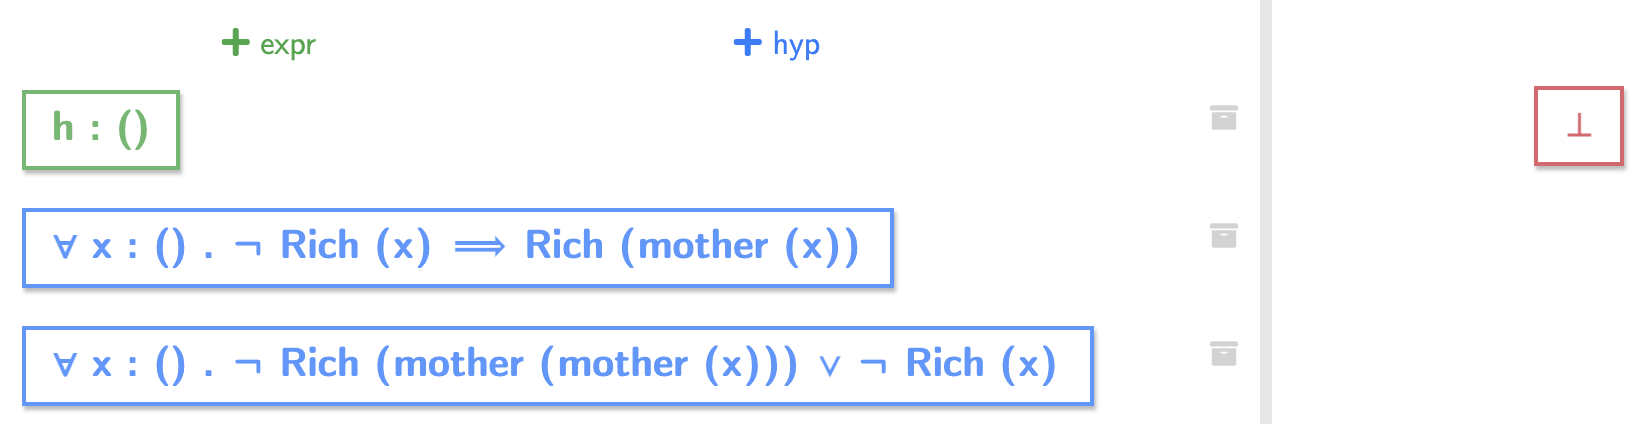
\includegraphics[width=1.3\textwidth]{edukera.png}}
\caption{The beginning of an example due to Edukera}\labfig{edukera}
\end{figure*}

It is too early to perform a detailed case study comparing our approach
to interactive theorem proving with others --- tactic-based,
declarative, {\em etc}\dots~This is due primarily to the fact that
our prototype is not mature enough; it cannot handle lemmas and
implements a limited formalism. However some examples allow to get a
glimpse of specificities and possible advantages of proofs by actions.

One such example is a small logical riddle, which we borrow from a
textual educational system, Edukera~\cite{edukera}. One considers a
population of people, with at least one individual $h$, together with a
single function $\mother$ and one predicate $\rich$. The aim is to
show that the two following assumptions are incompatible:
\begin{itemize}
\item[(1)] $\forall x. \neg\rich(x)\lor \neg\rich(\mother(\mother(x)))$,
\item[(2)] $\forall x. \neg\rich(x) \limp \rich(\mother(x)).$
\end{itemize}
The original goal thus corresponds to the illustration of \reffig{edukera}.

It is quite natural to approach this problem in a forward manner, by starting
from the hypotheses to establish new facts. And a first point illustrated by
this example is that DnD actions allow to do this in a smooth and precise
manner. A possible first step is to bring $h$ to the first hypothesis, to obtain
a new fact:

\medskip
$(3) ~\neg\rich(h)\lor \neg\rich(\mother(\mother(h))).$
\medskip

\noindent Double clicking on this new fact yields two cases:
\begin{itemize}
 \item[(4)~] $ \neg\rich(h)$,
 \item[(4')] $ \neg\rich(\mother(\mother(h)))$.
 \end{itemize}
Let us detail how one solves the
second one.

By bringing 
$\neg\rich(\mother(\mother(h)))$ on the premise of $\forall
x. \select{\neg\rich(x)} \limp \rich(\mother(x))$
one obtains

\medskip
$(6) ~\rich(\mother(\mother(\mother(h)))).$
\medskip

The next step is a good example where the DnD is useful. By bringing
this new fact to the right-hand part of

\medskip
$(1)~\forall x. \neg\rich(x)\lor \neg\select{\rich(\mother(\mother(x)))}$
\medskip

\noindent
one immediately obtains a new fact

\medskip
$(7) ~\neg{\rich(\mother(h))}$.
\medskip

\noindent In other proof systems, this last step requires a somewhat intricate
tactic line and/or writing down at least the statement of the new fact.

One can then finish the case by combining $(7)$ and $(2)$ which yields
$$\rich(\mother(\mother(h)))$$ contradicting $(4')$. These two last steps each
correspond to a simple DnD. The other case, $\neg\rich(h)$, is quite similar.

Such a simple example is not sufficient to provide significant
metrics. Note however that once a user has understood the proof, the
riddle is routinely solved in less than a minute in Actema, which
seems out of reach for about any user in a tactic based prover. At
least as important is the fact that the proof can be performed without
typing any text, especially no intermediate statement. 


\section{Related Works}\labsec{related-work}


\subsubsection*{Subformula Linking}

Although the primary motivation is very practical, it benefitted a lot from
recent works in proof theory, especially \emph{deep inference}. A key step was
the discovery of the work of Kaustuv Chaudhuri~\cite{Chaudhuri2013} who had
noticed how subformula linking in deep inference could be used for proof
construction in linear logic. His variant of the calculus of structures was very
important for designing the rewrite rules which underly our system, and in
\refch{pbl} we analyse proof calculi based on our rules that are closer to his
original formulation. In more recent work~\cite{DBLP:conf/cade/Chaudhuri21} he
also deals with intuitionistic logic. Interestingly, some ideas like forward
proof steps or the use of colors appeared independently in his and our work. A
difference is that we give the possibility to link first-order terms in addition
to propositions, which is the basis for rewrite actions.


\subsubsection*{Canonical Proofs}

The idea of reducing a proof to a collection of links between its dual formulas
is not new, and can be traced back to the \emph{matings} of Andrews
\cite{1674698} in the context of automated deduction. Matings are \emph{sets} of
links covering all \emph{atomic} occurrences, and proofs are matings satisfying
certain conditions. Our work differs in that we are interested in
\emph{interactive} deduction, and thus consider links as a mechanism of
inference rather than a syntactic criterion to discriminate proofs. Then a proof
is better understood as a \emph{list} of links, and the atomicity constraint is
relaxed to gain expressivity, since the creation of links is offloaded to the
user instead of the search procedure.

Another line of work, starting with the \emph{proof-nets} of Girard
\cite{girard_linear_1987}, is concerned with the more fundamental problem of
\emph{proof identity}, which requires a canonical notion of proof object
\cite{strasburger-problem-2019}. In the case of unit-free multiplicative linear
logic, the absence of any form of duplication/sharing/removal mechanism allows
to completely characterize a proof-net by the set of its \emph{axiom} links. The
difference with matings is that correctness of a proof structure can be
checked in \emph{polynomial} instead of exponential time, because of the absence
of duplication.
% This is because adding
% additives or exponentials, which can encode intuitionistic and classical logic,
% requires additional structure to represent uses of weakening and contraction.
% The \emph{combinatorial proofs} of Hughes \cite{Hughes_2006}
% \cite{heijltjes_intuitionistic_2019} are examples of polynomially-checkable
% proof objects exhibiting such structure, and have recently been extended to
% handle first-order classical quantifiers \cite{hughes2019firstorder}
% (intuitionistic quantifiers are still an open problem).
% This compartmentalization of axiom links and structural rules resembles the
% distinction between interaction phases and manual applications of {\rnmsf{conn}}
% and {\rnmsf{wkn}} in \sys{DISL^0}, which is itself inspired by the
% \emph{decomposition theorem} of deep inference formalisms.
% Another approach to canonicity is to consider a generalization of focused proofs
% called \emph{maximally multi-focused proofs}, which have been proven isomorphic
% to compact representations of proofs such as proof-nets
% \cite{ausiello_canonical_2008} and expansion tree proofs
% \cite{chaudhuri_multi-focused_2016}. We conjecture that our system \sys{ISL^1_2}
% could be reformulated as a multi-focused proof system, where foci correspond to
% the linked formulas, and thus their number is restricted to exactly 2.
There is an analogy between the correctness criterions of proof-nets, and the
validity criterion of linkages:
\begin{itemize}
  \item they both identify a subset of valid objects among a larger set of
  structures characterized by links on formulas;
  \item they both allow many different \emph{sequential} readings, that is
  sequent calculus proofs for proof nets, and deep inference, CoS-style proofs
  for linkages\sidenote{Note that invalid linkages still give rise to CoS-style
  \emph{derivations}, but not \emph{proofs} since they do not end with $\top$.
  The incorrect proof structures of Girard are in a sense more parallel as they
  cannot always be mapped to correct sequent calculus derivations.}.
\end{itemize}
Hence, our approach to subformula linking seems to exhibit some properties of
canonical proofs, but at the level of \emph{partial proofs}: valid linkages make
for \emph{compact-parallel-spatial} representations of inferences, whose
operational meaning is given by their \emph{detailed-sequential-temporal} CoS
derivations.


% More
% broadly, we envision a generalization of the linking method to any set of
% subexpressions, which might or might not be equivalent or have equivalent types,
% depending on the semantics of the action under consideration. Such a generalized
% method might be dubbed \emph{``link inference''}. Subformula linking then
% corresponds to a particular kind of action, which justifies any occurrence of
% proposition given another known, unifiable proposition.

\subsubsection*{Window Inference}
We have already mentioned Proof-by-Pointing, which was part of the CtCoq and
Pcoq efforts \cite{amerkad-mathematics-2001} to design a graphical user
interface for the Coq proof assistant. Another contemporary line of work was the
one based on \emph{window inference}, initially pioneered by P.J. Robinson and
J. Staples. In \cite{robinson-formalizing-1993}, window inference is described
as a general proof-theoretical framework, which aims to accomodate for the
pervasive use of \emph{equivalence transformations} throughout mathematics and
computer science.

% In \cite{robinson-formalizing-1993}, they describe it as a new kind
% of proof-theoretic framework, which aims to accomodate for the pervasive use of
% \emph{equivalence transformations} throughout mathematics and computer science.
% For this purpose, it provides facilities for describing how to focus on specific
% subexpressions, and perform transformations on them that preserve a given
% equivalence relation, while keeping and exploiting information from the context
% where they occur. It is noted in \cite{grundy-window-1991} that the framework
% can be extended to more general relations like preorders, which might typically
% be used to capture the entailment relation of a logic.
Window inference has been used both for general-purpose logics like
HOL \cite{grundy-window-1991}, and in more specialized settings like
program refinement \cite{grundy-window-1992}. It naturally lends
itself to integration in a graphical user interface
(\cite{langbacka-tkwinhol-1995}, \cite{goos-tas-2000}), where the user
can \emph{focus} on a subexpression by clicking on it. One is then
presented with a new \emph{graphical} window, holding the selected
expression as well as an extended set of hypotheses exposing
information inferrable from the context of the expression. The user
can pick from a list of valid transformations to be applied to the
expression, before closing the window. This propagates the
transformations to the parent window by replacing the old
subexpression by the new one, without modifying the surrounding
context.

This process is quite reminiscent of the rewriting produced by our DnD
actions.  One key difference is that window inference rules can be
applied stepwise, while we choose to hide the sequence of rules that
justifies a DnD. The window inference approach gives to the user a
precise control of the transformations to be performed and thus could
inspire interesting extensions of our work.

% This is because
% DnD actions embody the specific intent of justifying an \emph{expression} by
% another \emph{user-specified} expression, which is either assumed to be, or
% trivially equivalent. In contrast, window inference is about justifying the
% \emph{equivalence} of an expression to another, \emph{not yet specified}
% expression. Another way to see it is that our ``link inference'' technique aims
% to capture the process of \emph{applying} some knowledge, while window inference
% provides an interface for the \emph{construction} of new knowledge. They thus
% appear as equally valid and even complementary approaches, that could benefit
% from being implemented in the same interface.

\subsubsection*{Tangible Functional Programming}
We noticed an interesting connection with the work of Conal Elliott on
tangible functional programming \cite{elliott-tangible}. His concept
of \emph{deep application} of $\lambda$-terms seems related to the
notion of subformula linking, when viewing function and product types
as implications and conjunctions through the formulae-as-types
interpretation. He also devised a system of basic combinators which
are composed sequentially to compute the result of a DnD, though it
follows a more complex dynamic than our rewrite rules. Even if the
mapping between proofs and programs is not exact in this case, it
suggests a possible interesting field of application for the
Curry-Howard correspondance, in the realm of graphical
proving/programming environments.

\subsubsection*{Other Gestural Proof Systems}
There are other proof systems which include drag-and-drop features. Two of them
are the KeY Prover \cite{ahrendt-using-2016} and TAS \cite{goos-tas-2000}. TAS
is a window inference system tailored for program refinement, and uses DnD
actions between an expression and a transformation, in order to apply the latter
to the former.
%This is obviously different from our use of DnD between entities
%of the same kind, and can be explained by the comparison made in the previous
%paragraph.
As for the KeY Prover, its usage of DnD overlaps only a very small
portion of usecases that we hinted at in \refsec{edukera}, namely
the instantiation of quantifiers with objects.

We can also mention the recent work of Zhan et
al. \cite{zhan-design-2019}. They share with us the vision of a proof assistant
mainly driven by gestural actions, which requires far less textual inputs from
the user. However, they only consider point-and-click actions, and rely on a
text-heavy presentation at two levels:
\begin{enumerate}
  \item the proof state, which is a structured proof text in the style of Isar~\cite{isar};
  \item the proof commands, which can only be performed through choices in textual menus.
\end{enumerate}

% The latter can be useful to integrate specific actions which do not fit
% naturally in the gestural paradigm. But because basic reasoning with logical
% connectives and equations occurs so often in virtually any proof, we believe it
% deserves a special treatment in the interface, and our work shows that
% drag-and-drop gestures can be used efficiently for that purpose. This was
% already a concern in \cite{amerkad-mathematics-2001}, where PbP is seen as a
% mean to \emph{``increase the bandwidth between the user and the logical
% engine''}, along with other devices like advanced graphical notations. The
% authors also described how PbP is partially compatible with the production
% \emph{in real time} of a proof text in quasi-natural language, thus close to an
% Isar proof. We conjecture that our drag-and-drop mechanism also has this
% capability, and in fact solves some of the problems induced by the limitation of
% PbP to a single selection.


\subsubsection*{Explicit Proof Objects}

Finally let us mention various recent implementations proposing various ways to
construct proofs graphically: Building Blocks~\cite{buildingblocks}, the
Incredible Proof Machine~\cite{blanchette-visual-2016},
Logitext\sidenote{\url{http://logitext.mit.edu/main}} and Click \&
coLLecT~\cite{clickcollect}. In particular, Logitext and Click \& coLLecT
exploit the same idea of associating click actions on head connectives to
inference rules in sequent calculus. But these systems focus more on explicating
the proof object than on making its construction easier.


% \section{Conclusion and Perspectives}
% This work started as a very practical effort. Discovering and
% understanding the links with more theoretically grounded approaches,
% and especially deep inference, made us aware that there may be more
% proof theoretical depth to this idea than we first thought. But, most
% importantly, adapting the logical rules and tools of deep inference to
% the practical question we encountered, allowed us to structure our
% proposal and to define the ``right'' behavior for the system. We were
% able to extend the deep inference approach to the use of
% equalities~\refsec{equality}, which may be an originality of this
% work. It seems imaginable to proceed similarly with other mathematical
% relations. 

% More generally, we hope that our treatment of equality can be the
% start for providing graphical or gestural tools to perform algebraic
% transformations of expressions (be there in the conclusion or in
% hypotheses). As mentioned above, Window Inference could serve as an
% inspiration here. This seems promising to us, since describing such a
% transformation is notoriously tedious when using textual commands.

% Even a small prototype allowed us to experiment on some non-trivial
% examples and to make some first encouraging experiences. In various
% cases, like the one described in section~\refsec{edukera}, we have
% observed shorter or more straightforward proofs than in textual
% provers. Another nice point is that some syntactical details, like the
% name of proof tactics become irrelevant in the gestural setting. More
% generally, we feel that using such a system, one may indeed develop a
% good intuition for the behavior of the logical items. But this is
% obviously a user interface or user experience question which is too
% early to quantify. Also, some novel questions appear when implementing
% such a graphical system: what are the good user interface choices, how
% to obtain a good look-and-feel, what visual feedback the system should
% provide\dots

% On the other hand, we should acknowledge that certain styles of proofs,
% where a large number of subcases can be immediately solved through the
% same short textual tactic sequence, may be less well suited for the
% gestural approach (the SSReflect~\cite{SSR} dialect for Coq is very
% well suited for such cases).


% Among future lines of work, it will be interesting to explore how some
% automation fits into this framework. One example is the \emph{point-and-shoot}
% paradigm of \cite{PbP}. But the DnD feature could open up new possibilities,
% like having the system perform some automated deduction to prove equivalences or
% implications between the two squared formulas (which would thus no longer be
% required to be strictly equal or unifiable).

% Another obvious and important point to be tackled next is to provide a
% smooth way to invoke a library of lemmas in a graphical proof. We
% believe this could raise some interesting questions.

% An also promising line of work is to extend our approach to classical
% logic. A point being that the graphical setting could smoothly handle
% multiple conclusions with less spurious overhead than text commands.


% An important difference with the days of the
% pioneering work on proof-by-pointing is that developers can now rely on
% powerful and standardized libraries, which make the construction of
% user interfaces much faster and easier, giving new room for
% experimentation and proposals. But bringing everything together in
% simple commands remains a complicated theoretical and development task.